\chapter{Results and Discussion}\label{ch:results}

Below, we present the results of our analysis. We concentrate on output radiation (photon-flux density), as a function of frequency. Unless specified, the input parameters for the calculations are (unitless) drive frequency $\Omega= 12$, lattice parameter $\epsilon = 5$, modulation amplitude $\delta \epsilon = \epsilon/4$. All of the plots in our results were produced using the Python program found in the author's public GitHub repository \cite{Github_Repository}.

\section{One driven SQUID embedded in coplanar waveguide (CPW) }\label{sec:results_both_sides}
%
Below, in Fig. \ref{fig:naked_SQUID}, we show the output radiation emitted by a single SQUID embedded in a CPW. This is in contrast to previous work \cite{Johansson2009}, from which we borrow input parameters. We obtain a similar result, producing the distinctive one-mirror parabolic DCE shape described in \cite{Lambrecht1996}. One important distinction from the work cited is that the SQUID is embedded in a CPW, as opposed to terminating the CPW with a SQUID (effectively making the mirror semi-transparent as opposed to perfectly reflecting), radiation travels away from the mirror on both sides. A slightly higher overall photon-flux density is produced. 
%
%
%
\begin{figure}
    \centering
    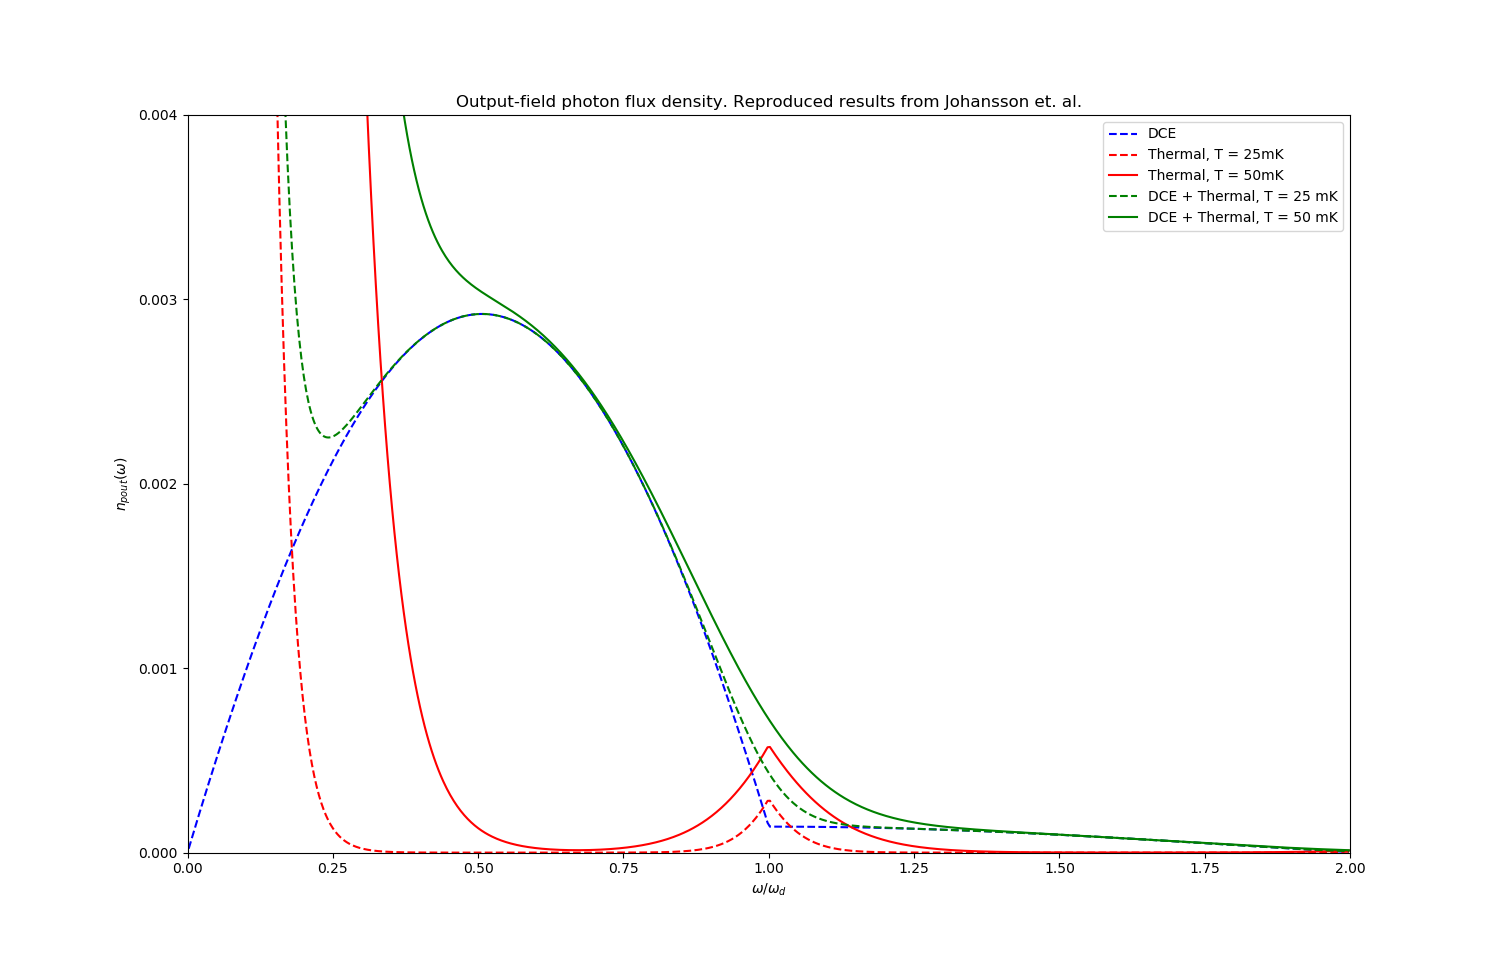
\includegraphics[width=\textwidth, keepaspectratio]{figures/intro/Johansson2010_reproduced.png}
    \caption{Reproduced results from \protect\cite{Johansson2010}, for radiation generated by a single SQUID. Here, the field only propagates on one side of the SQUID.}
    \label{fig:reproduced_Johansson_2}
\end{figure}
\clearpage
%
\begin{figure}[h]
    \centering
    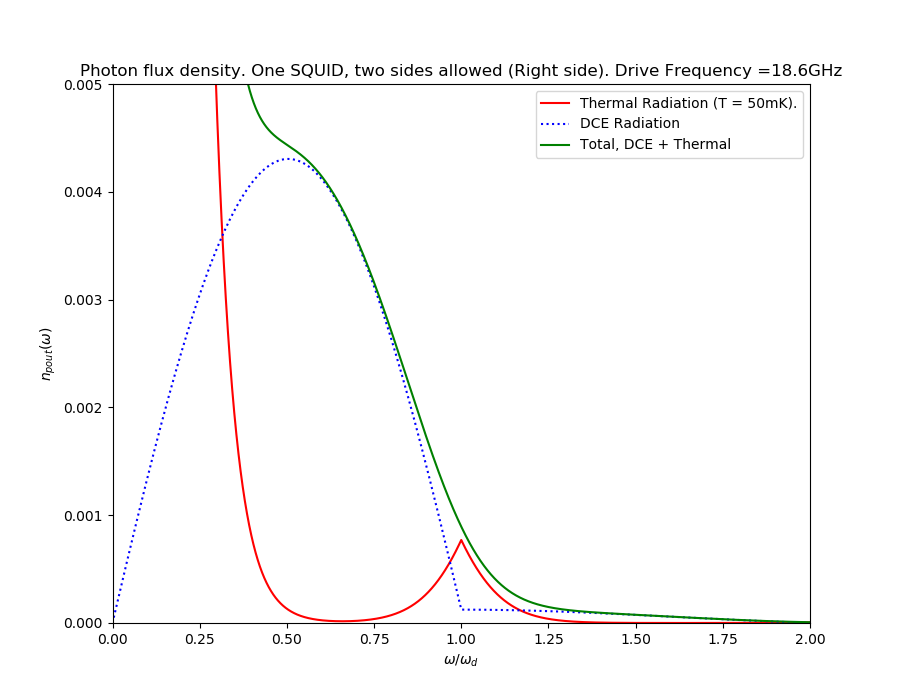
\includegraphics[width=0.9\textwidth, keepaspectratio]{figures/results/Naked_SQUID_right.png}
    \caption{Output radiation for one single semi-transparent SQUID. We allow both sides of the SQUID to have incoming/outgoing radiation. Horizontal axis is normalized with drive frequency $\omega_d$. Left/right output radiation is symmetric.}
    \label{fig:naked_SQUID}
\end{figure}
%
\clearpage
\newpage
\section{One SQUID embedded in lattice}\label{sec:results_one_active}
We now discuss results of our own model for a periodic SQUID lattice. Forbidden regions (see Section \ref{subsec:kpsol}) are shown in light blue. For these regions, no radiation (DCE or thermal) travels outside of the lattice. Detectable radiation is produced only within allowed regions.

For the following figures (\ref{fig:one_SQUID_active}-\ref{fig:one_SQUID_active_e_14_T_50}), only one SQUID is drive at a frequency $\Omega =12$, in a periodic lattice with different lattice parameters $\epsilon$. Different radiation patters emerge by changing the drive frequency and lattice parameter. Figure \ref{fig:one_SQUID_active}, shows the radiation produced by one single driven SQUID in a lattice $\epsilon=5$ which corresponds to physical lattice separation of about 2.21mm.
%
\begin{figure}
    \centering
    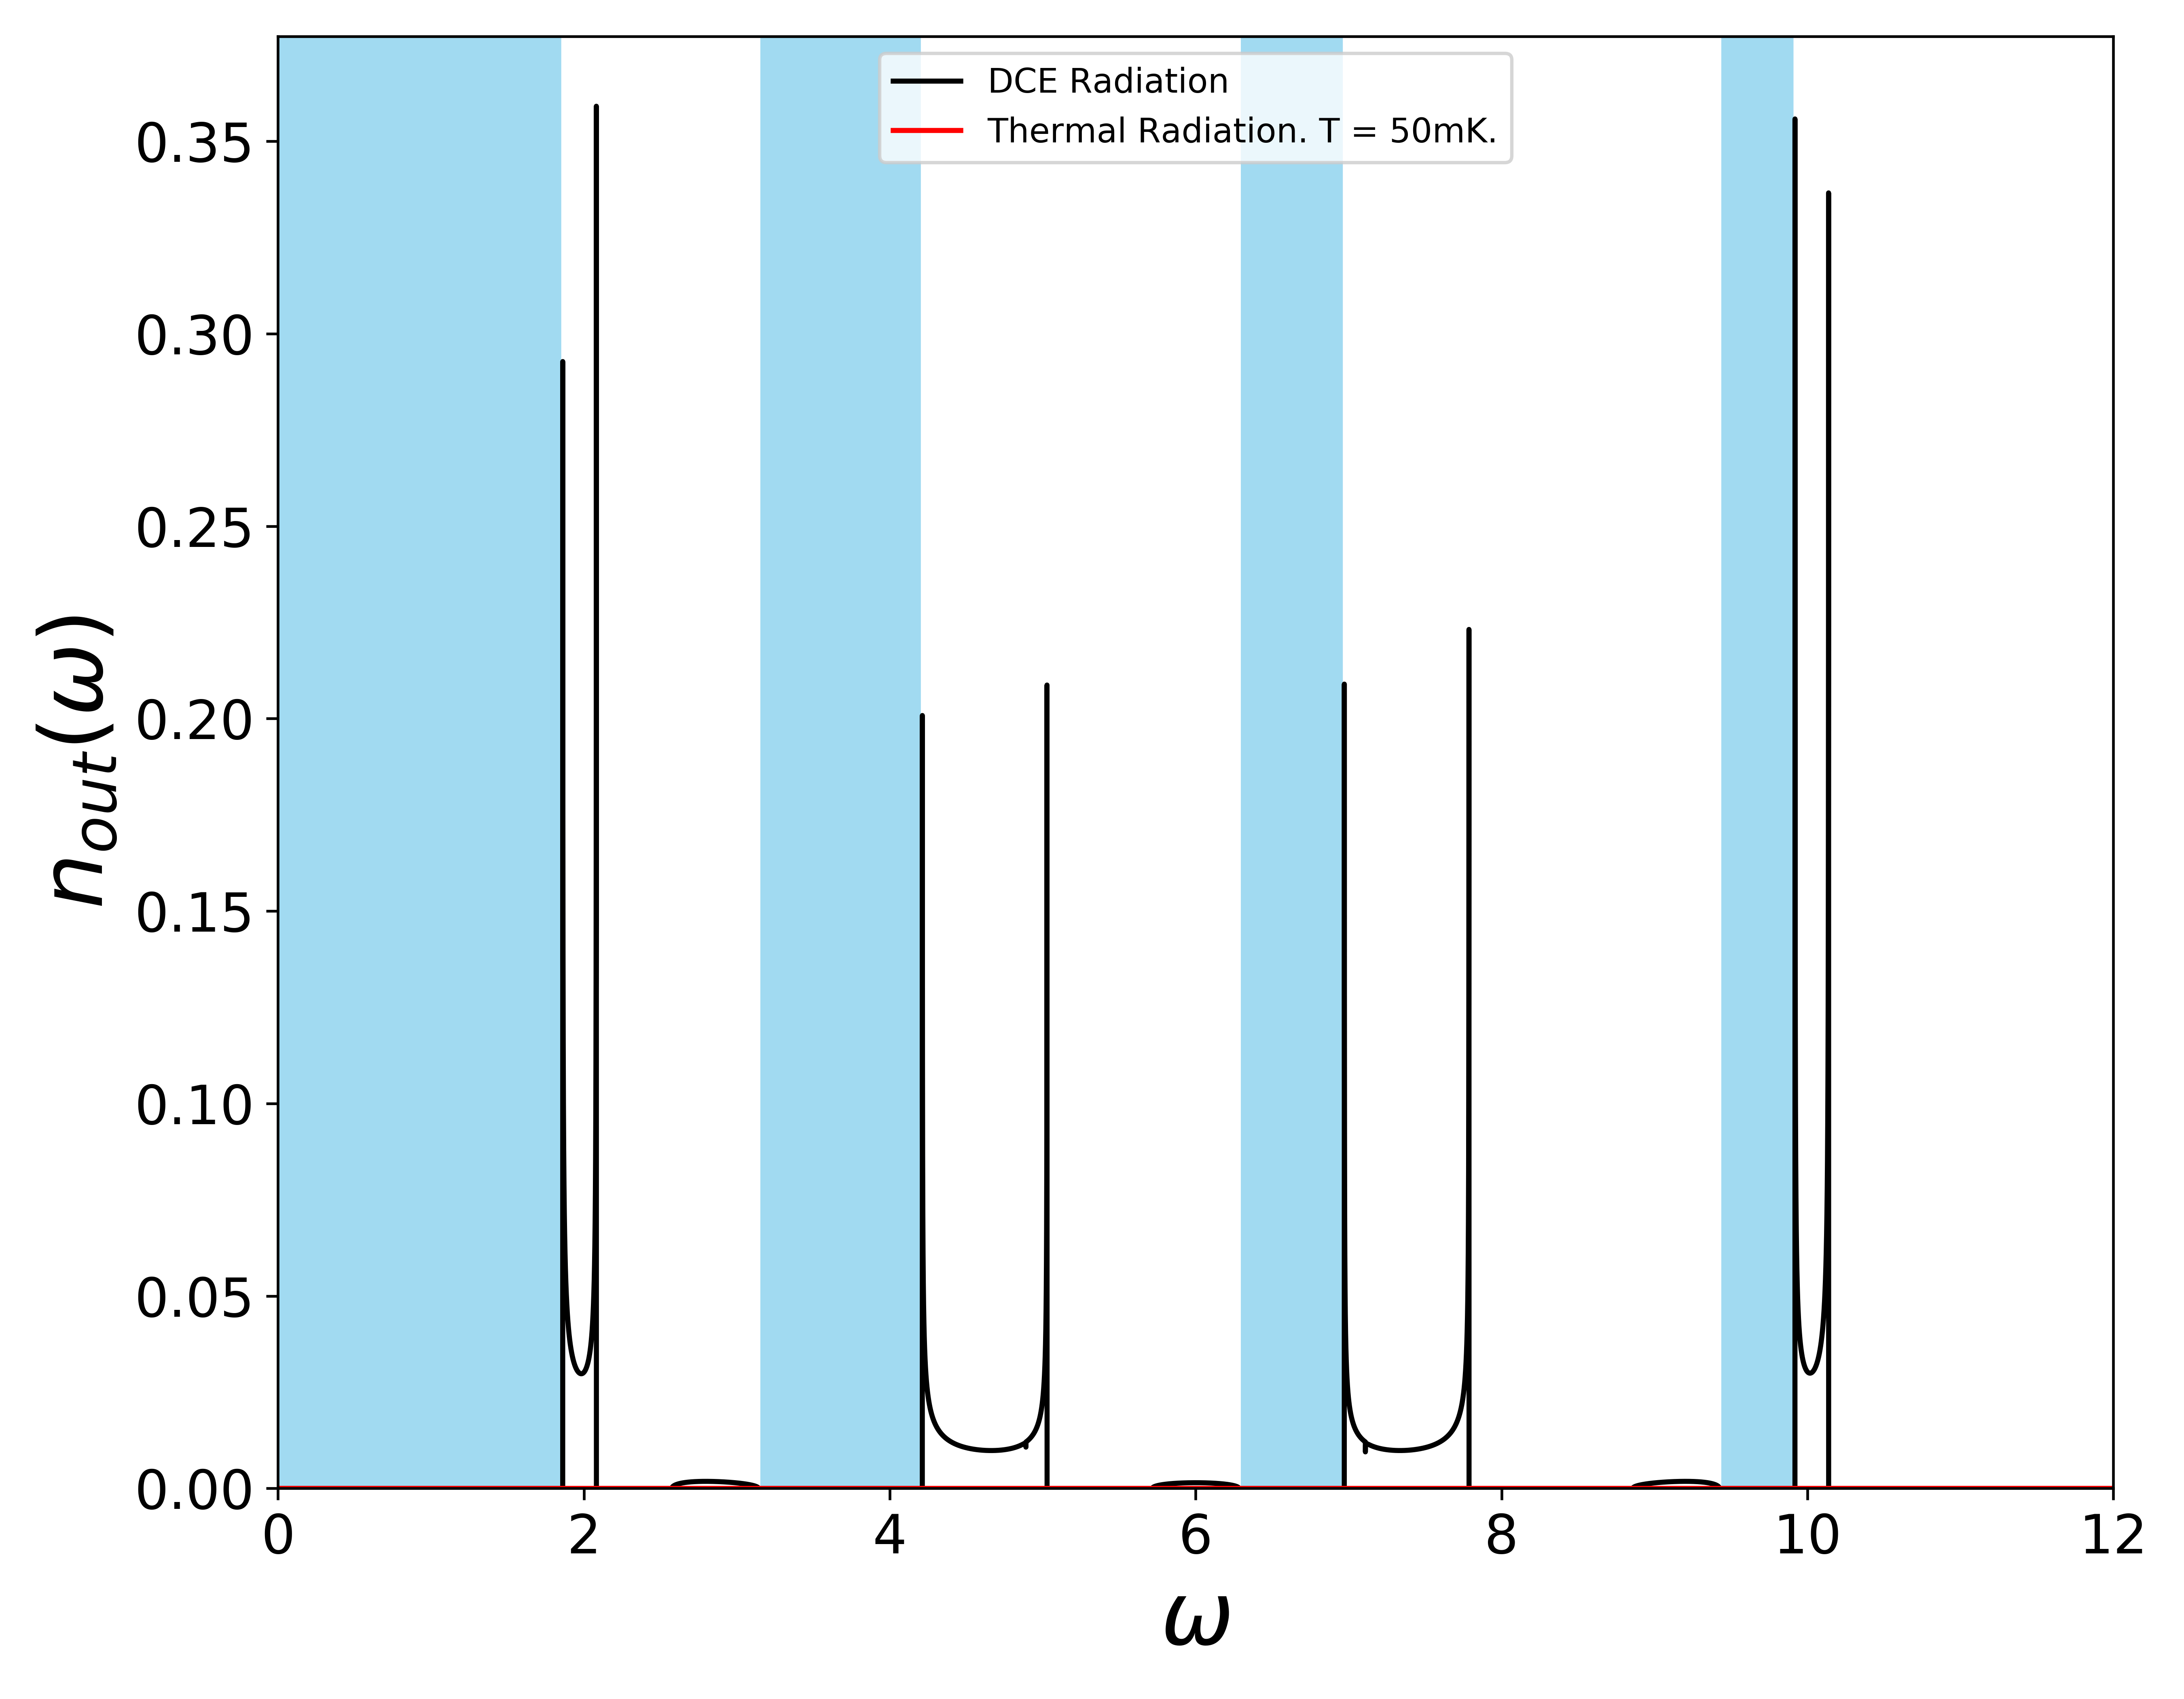
\includegraphics[width=\textwidth, keepaspectratio]{figures/results/one_SQUID_active.png}
    \caption{Output radiation for one single driven SQUID embedded in lattice with 50 static SQUIDs to either side. Input parameters used: $\Omega=12$, $\epsilon=5$.}
    \label{fig:one_SQUID_active}
\end{figure}
%
\newpage
The radiation pattern changes dramatically compared to the one for a single SQUID between CPWs, when no lattice is present (see Fig. \ref{fig:naked_SQUID}). The dramatic difference can be attributed to the presence of allowed and forbidden regions, as well as the change in the boundary condition due to the properties of Bloch functions, and the shape of the ground states of the field excited by the perturbation of such boundary conditions. A single SQUID surrounded by CPW would excite plane wave modes of the field, while when place in a lattice, the Bloch modes are excited instead.
%
\begin{figure}[h]
    \centering
    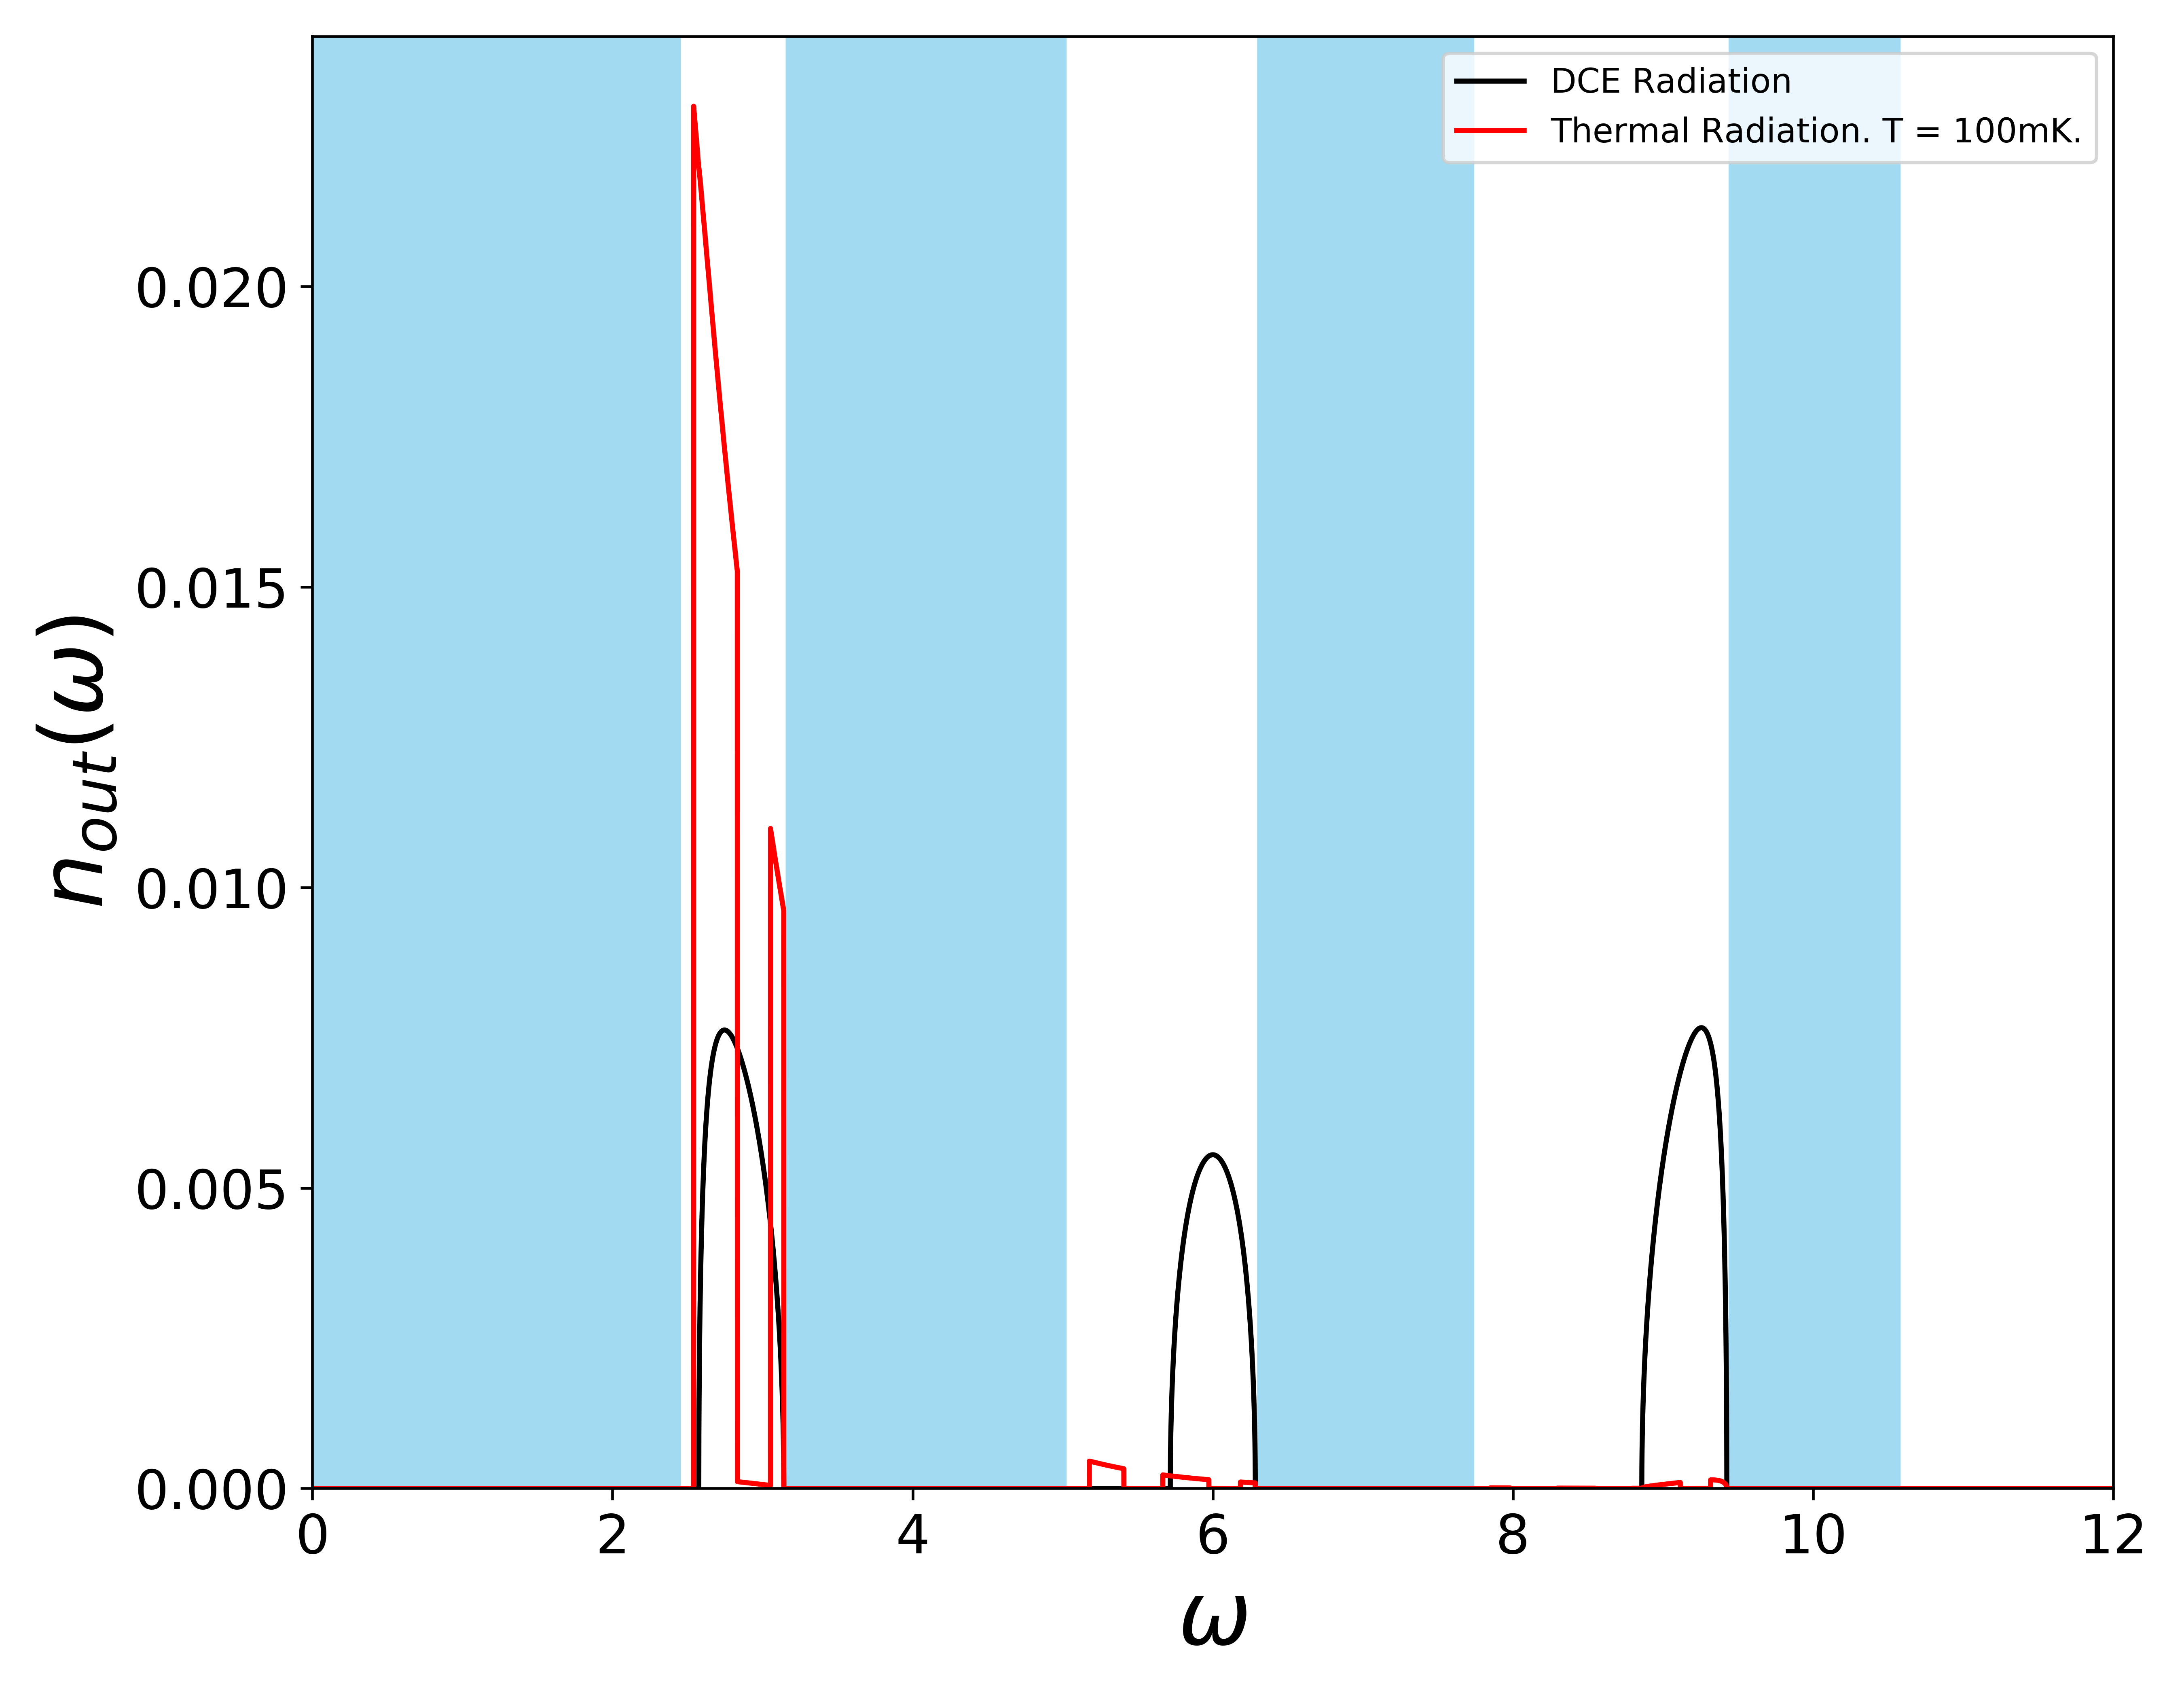
\includegraphics[width=\textwidth, keepaspectratio]{figures/results/one_SQUID_active_epsilon_14_100mK.png}
    \caption{Output radiation for one single driven SQUID embedded in lattice. Input parameters used: $\Omega=12$, $\epsilon=14$. A different band structure shows thermal contributions to the radiation. Temperature = 100mK.}
    \label{fig:one_SQUID_active_e_14_T_100}
\end{figure}
%
\newpage
Note that the presence of forbidden regions, particularly the region before the first allowed band, make it so the thermal radiation is filtered out. Since the input thermal radiation follows an inverse exponential relation for low frequencies (see Fig. \ref{fig:naked_SQUID}), the first forbidden region absorbs most of the thermal radiation. By changing the structure of the lattice to $\epsilon = 14$, the presence of thermal radiation can be observed, as well as well as different features in the DCE radiation (see Figure \ref{fig:one_SQUID_active_e_14_T_100}).
%
\begin{figure}[h]
    \centering
    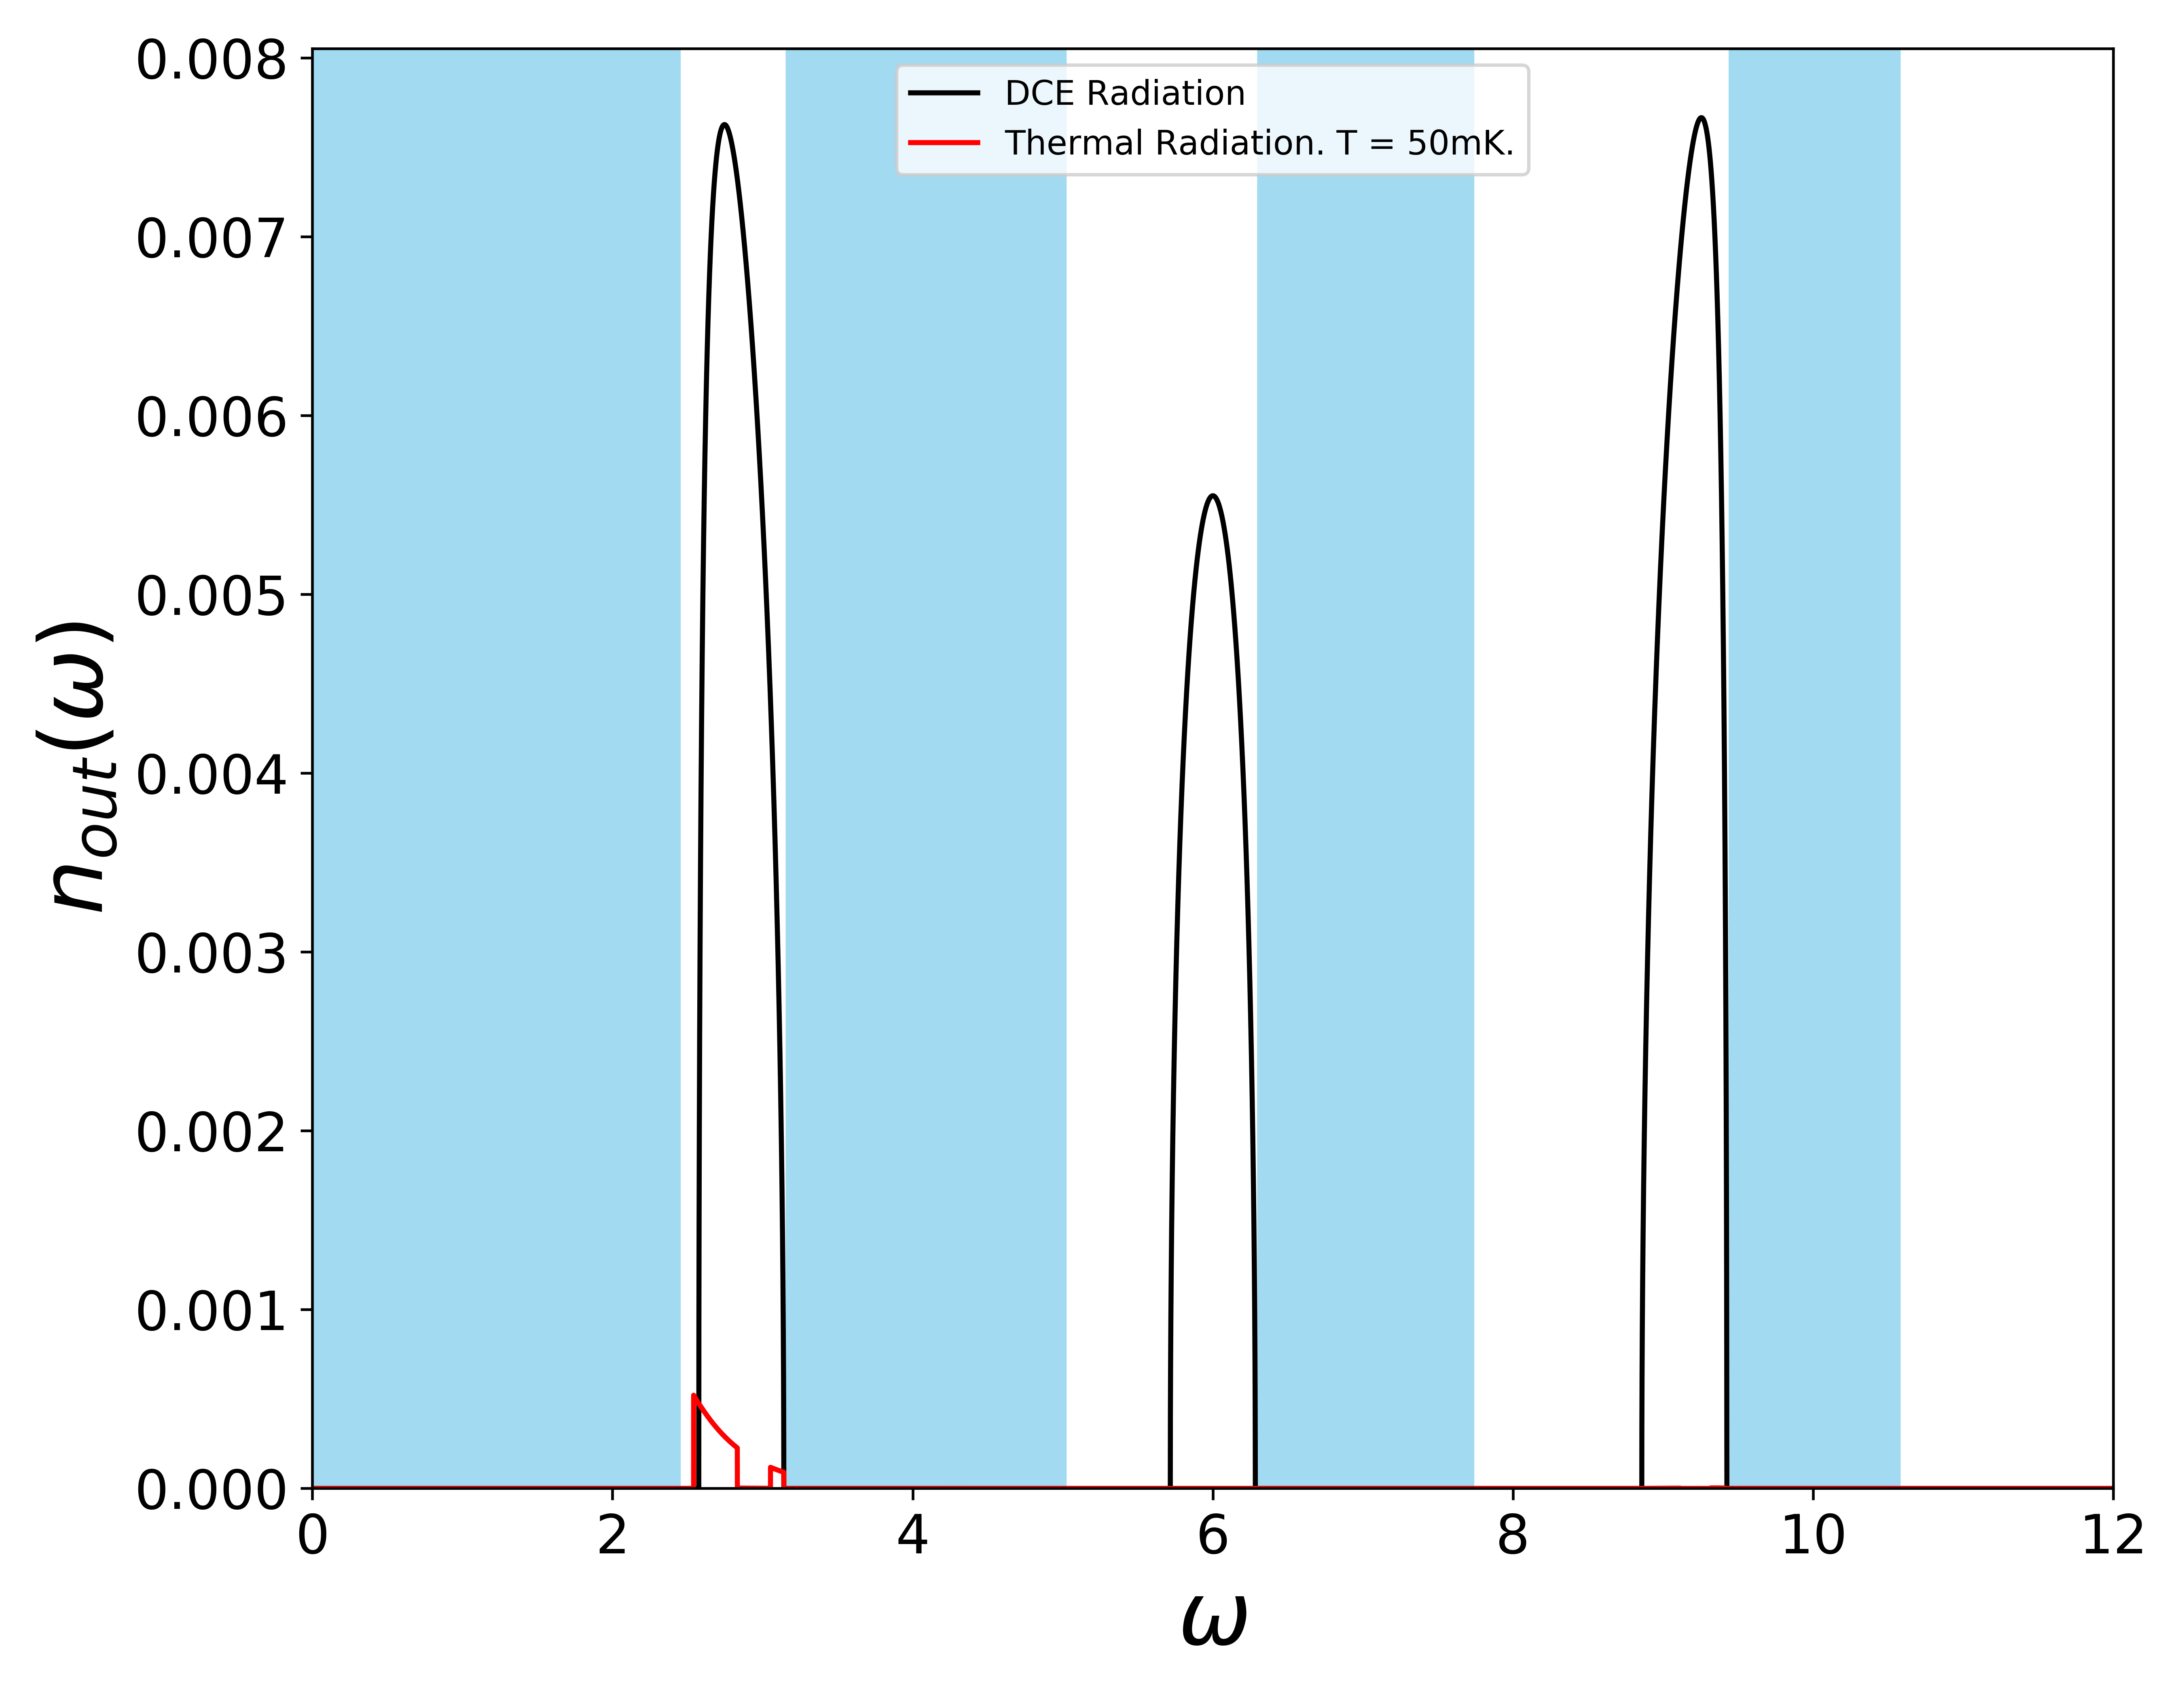
\includegraphics[width=\textwidth, keepaspectratio]{figures/results/one_SQUID_active_epsilon_14.png}
    \caption{Output radiation for one single driven SQUID embedded in lattice. Input parameters used: $\Omega=12$, $\epsilon=14$. A different band structure shows thermal contributions to the radiation. Temperature = 50mK.}
    \label{fig:one_SQUID_active_e_14_T_50}
\end{figure}
%

\newpage

Figure \ref{fig:one_SQUID_active_e_14_T_50}, shows how the distinct features of DCE radiation change when a different band structure is used (which is equivalent to changing the lattice parameter $\epsilon$) (see Fig. \ref{fig:one_SQUID_active}). Here, the radiation is closer to the familiar single-SQUID parabolic shape. Note how the features of DCE radiation are not localized in one allowed region but instead cover multiple regions. 

\section{All SQUIDs embedded in lattice}\label{sec:results_all_active}

The plots in this section correspond to the results of the case where all of the SQUIDs in a lattice with parameter $\epsilon$ are driven simultaneously (site-dependent phase $\varphi_n=0$) with frequency $\Omega$. We show the radiation spectrum for lattices of different sizes, with the size given by the number of SQUIDs in the lattice.

\begin{figure}[h]
    \centering
    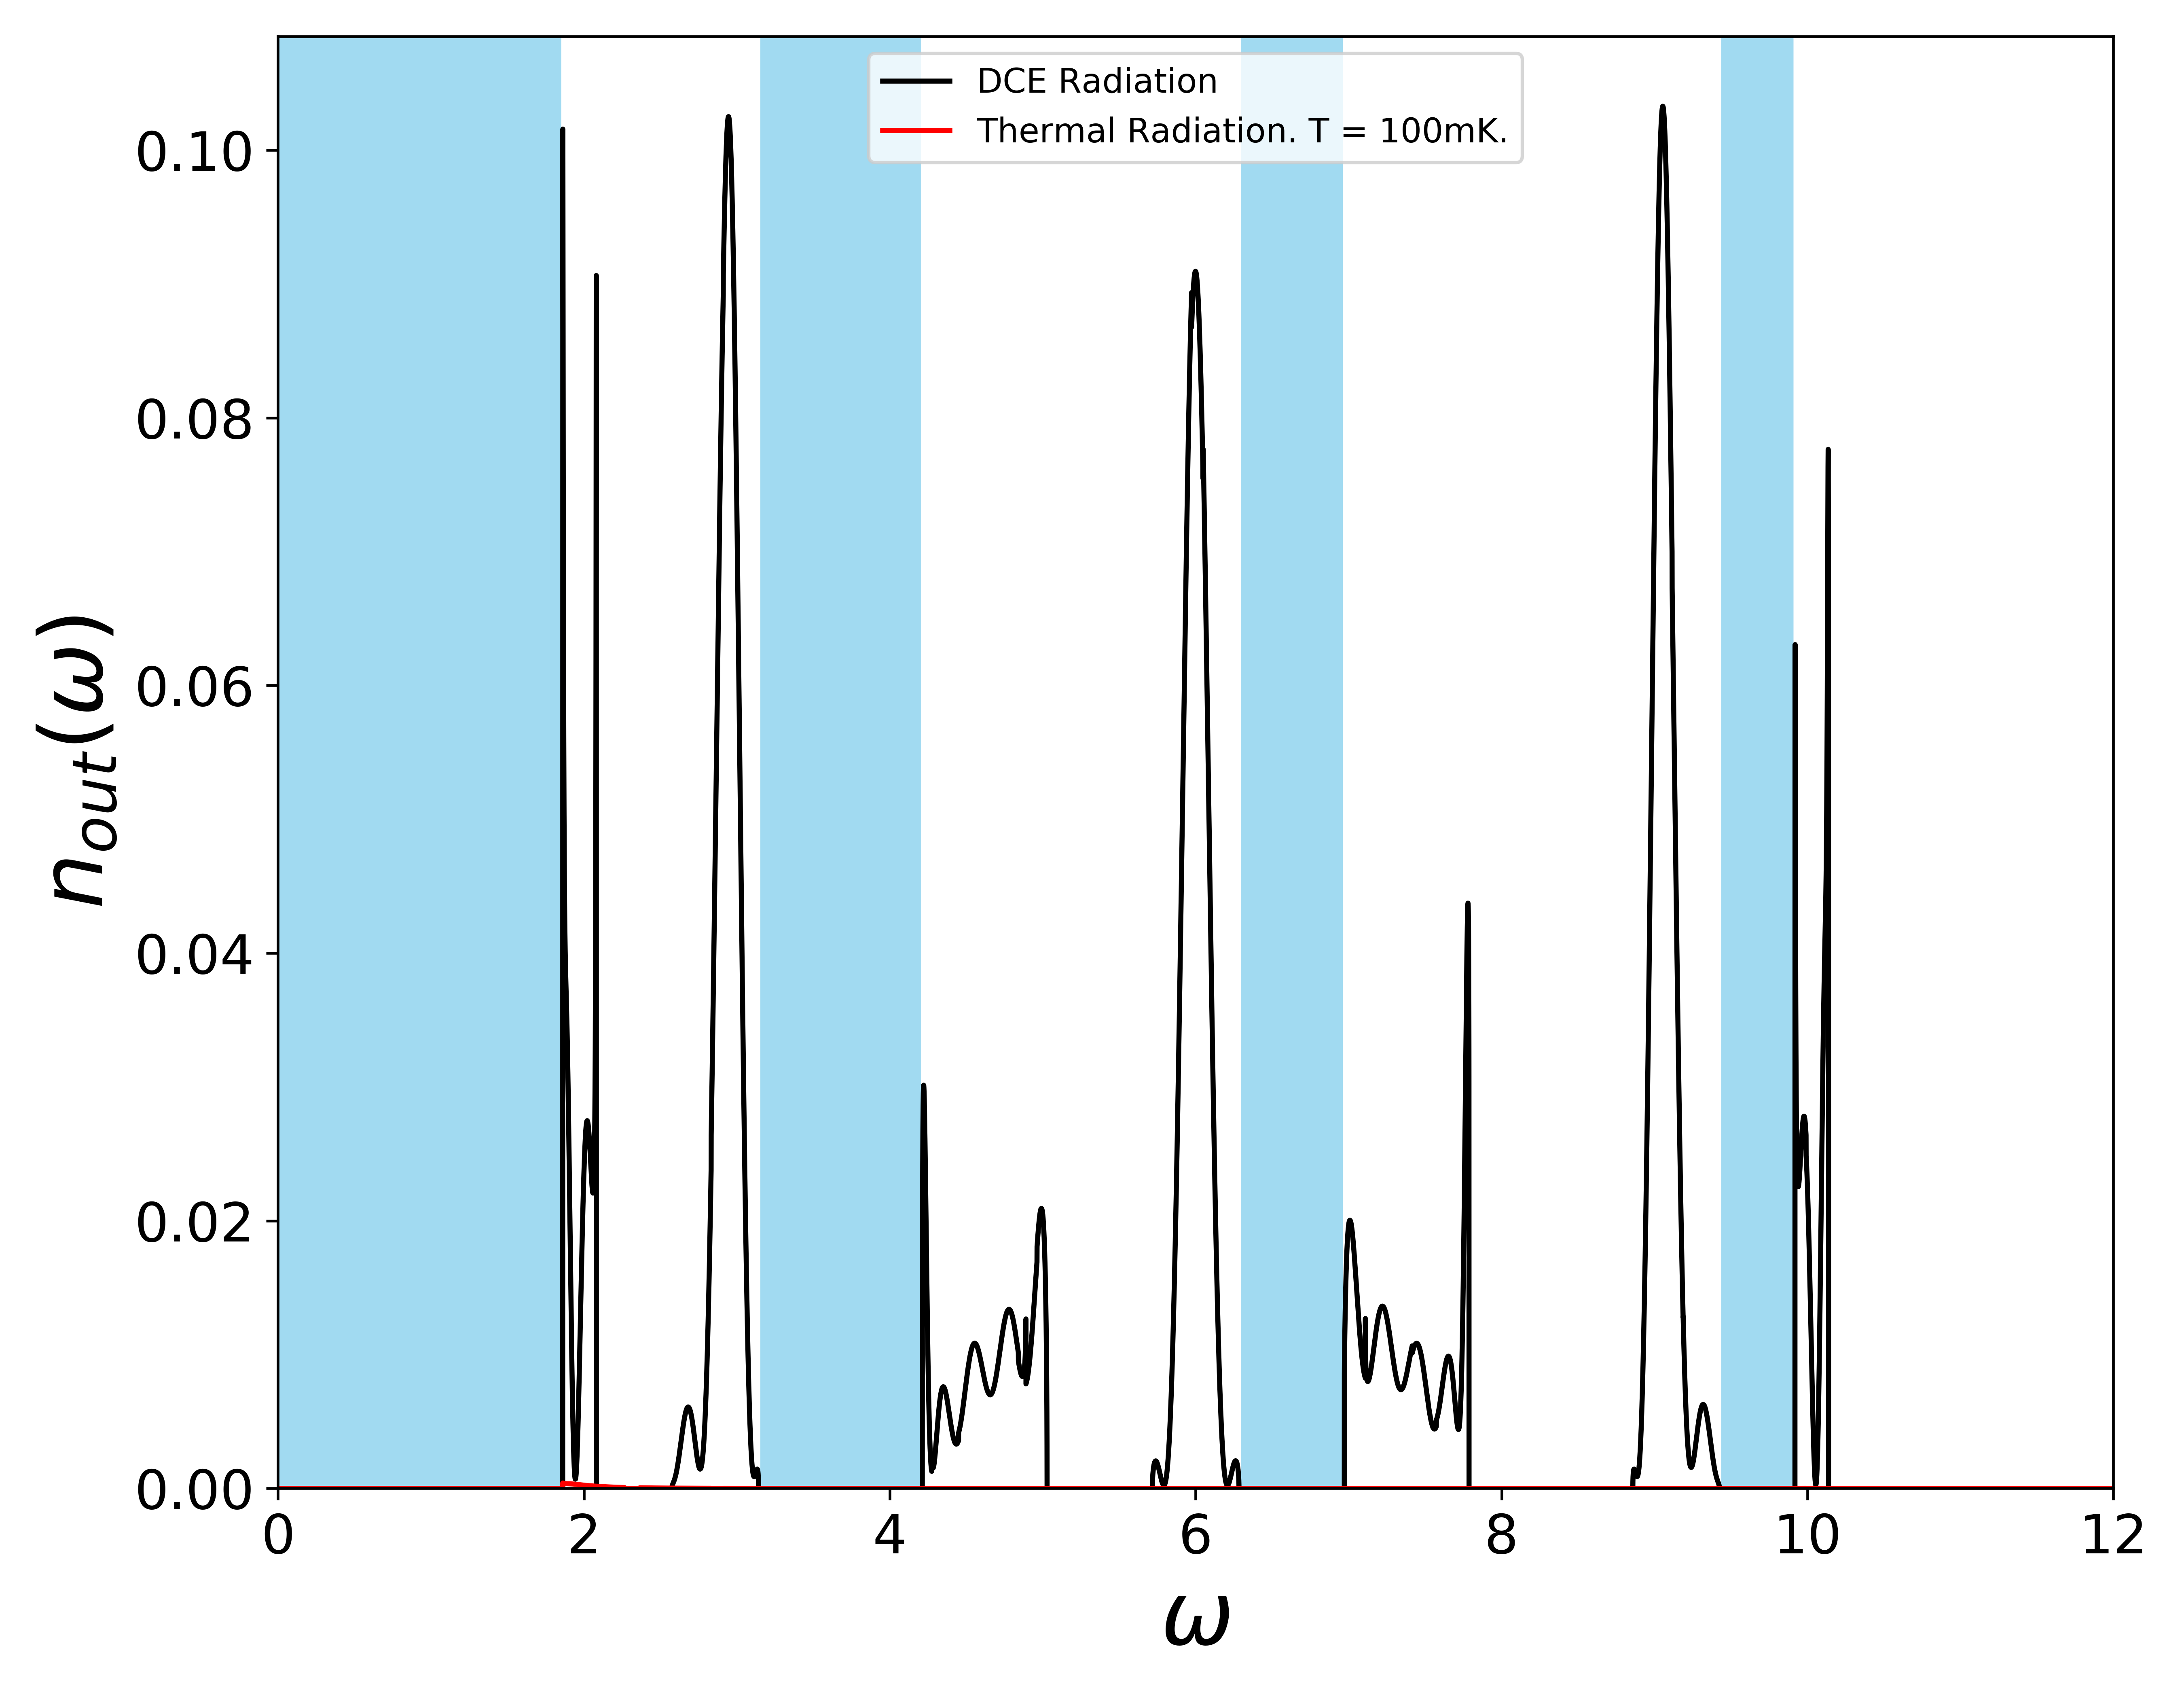
\includegraphics[width=\textwidth, keepaspectratio]{figures/results/10_SQUIDs_active.png}
    \caption{Output radiation for lattice of 10 driven SQUIDs. Input parameters used: $\Omega=12$, $\epsilon=5$. Complex radiation patterns arise when all SQUIDs are active.}
    \label{fig:10_SQUIDs_active}
\end{figure}
%
\begin{figure}[h]
    \centering
    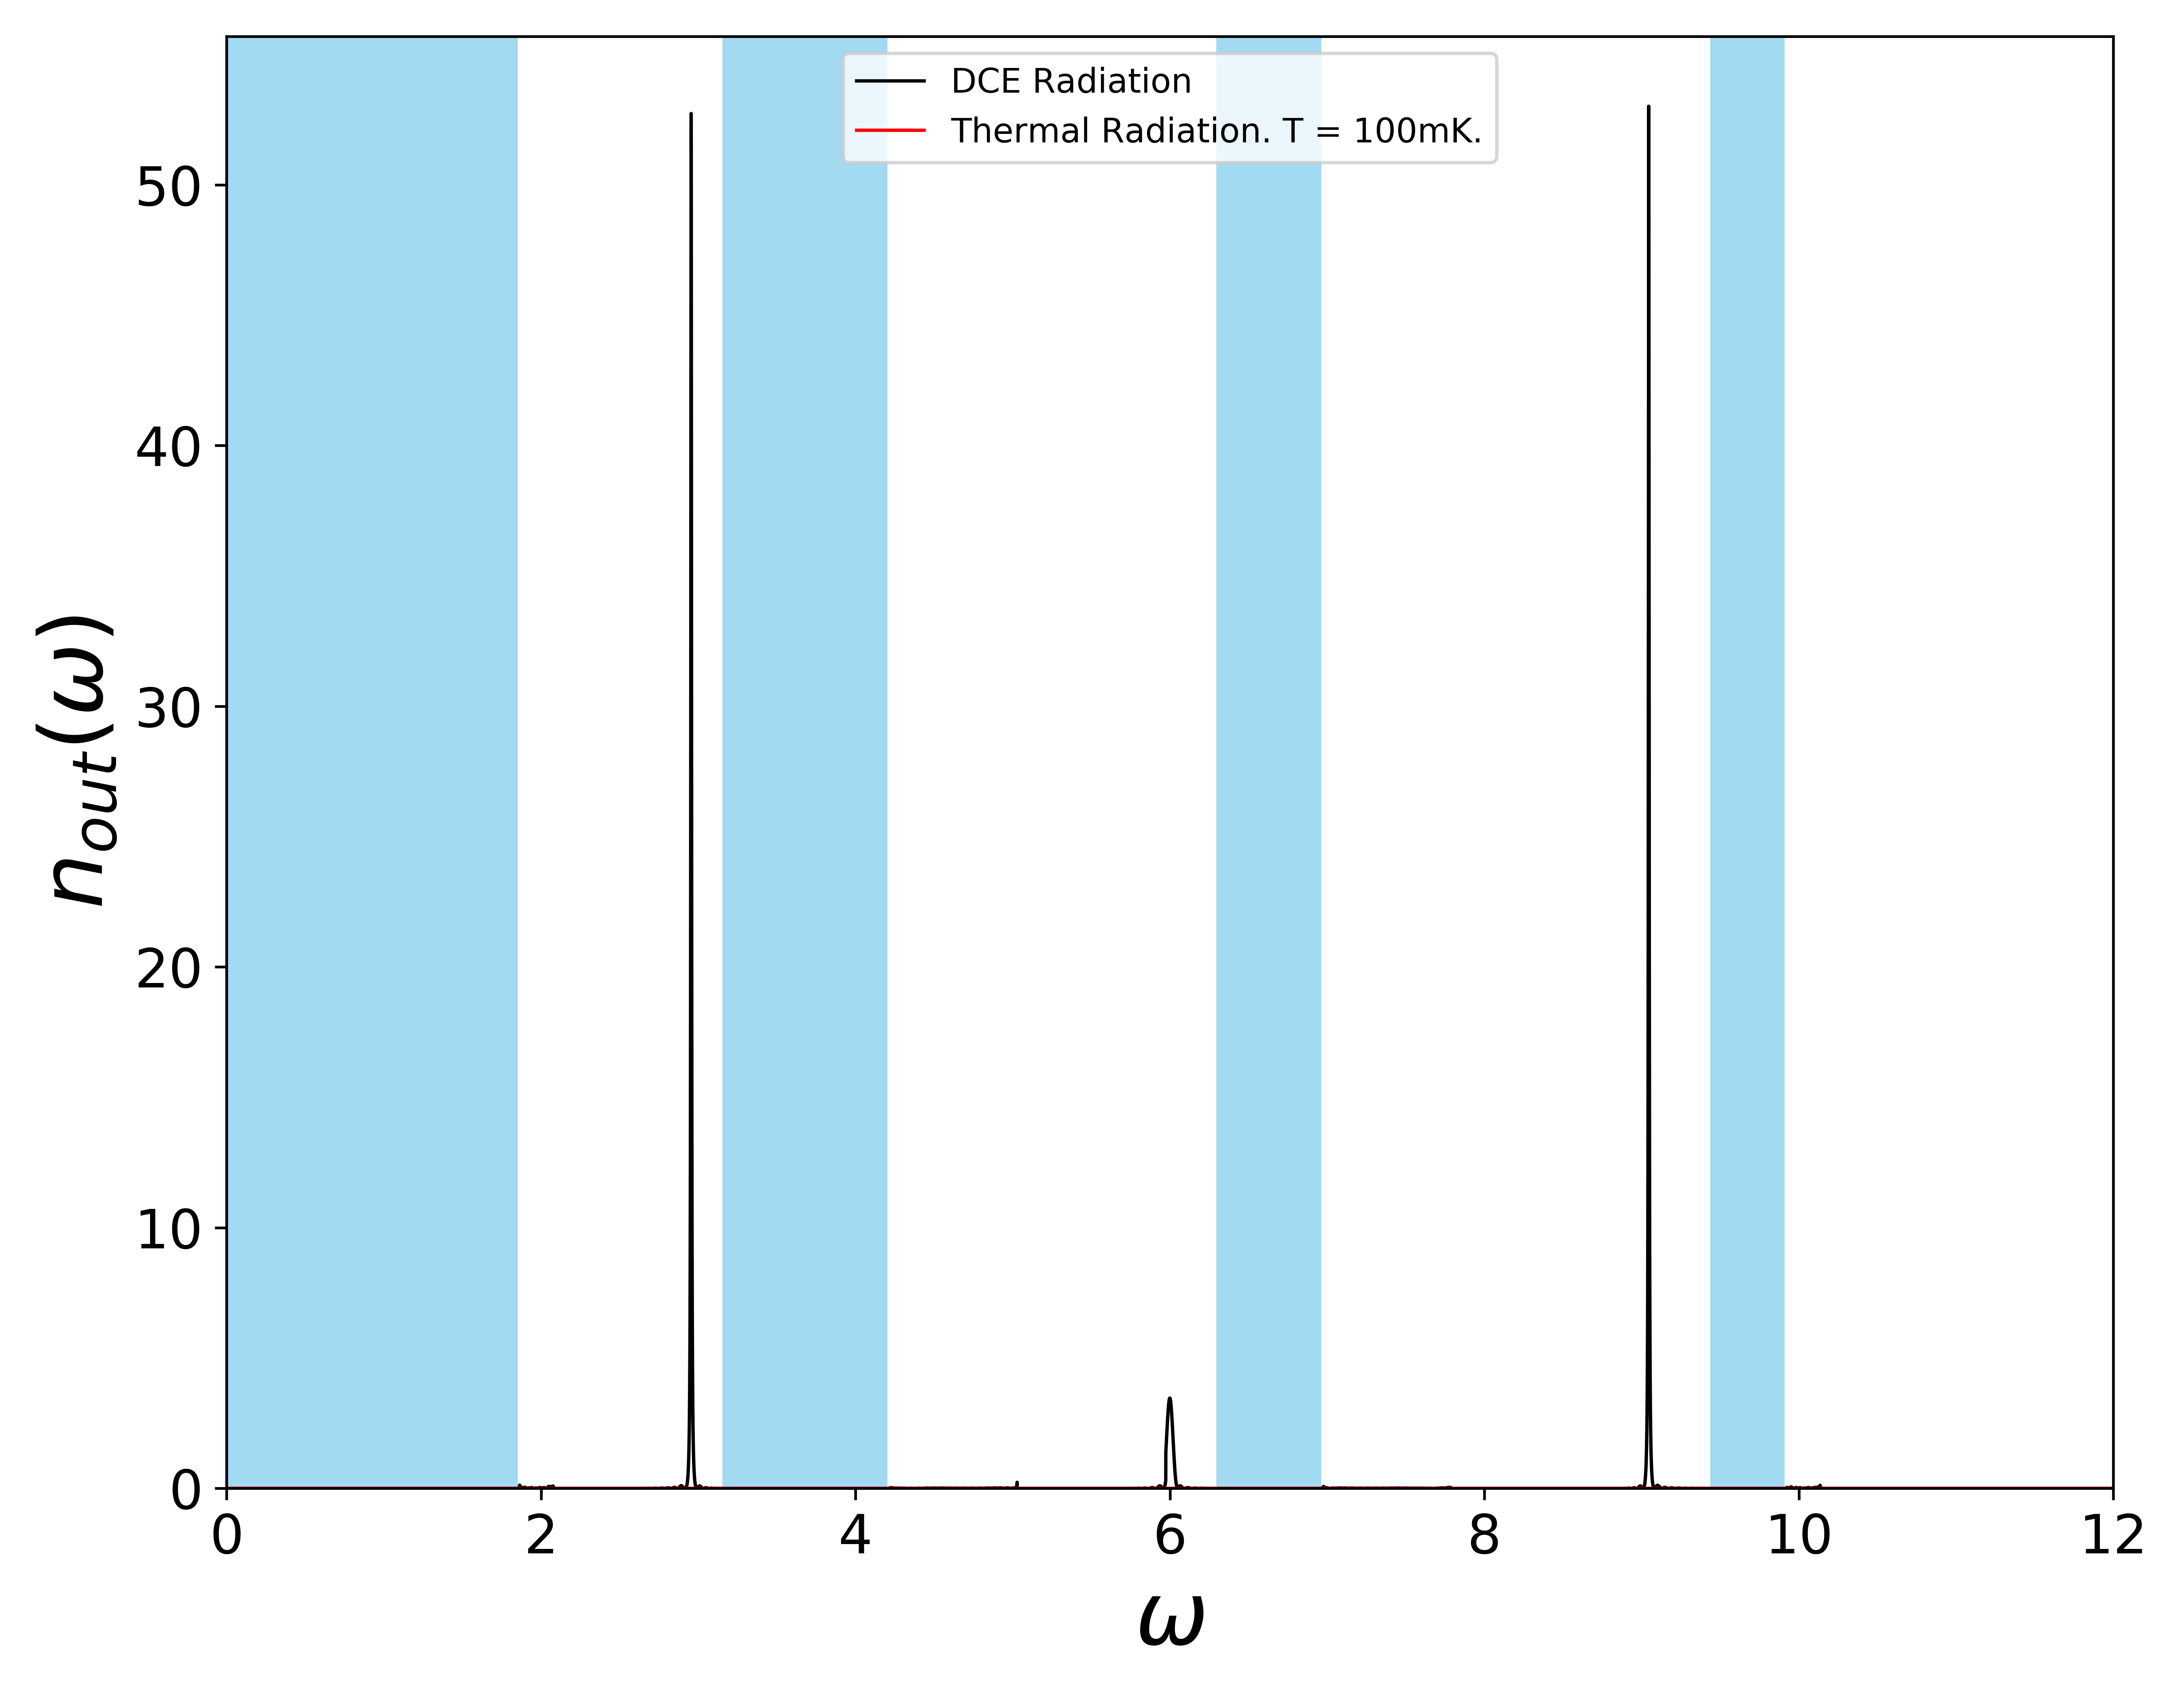
\includegraphics[width=\textwidth, keepaspectratio]{figures/results/50_SQUIDs_active.png}
    \caption{Output radiation for lattice of 50 driven SQUIDs. As we increase the number of SQUIDs, photon-flux density increases at narrow frequency ranges.}
    \label{fig:50_SQUIDs_active}
\end{figure}
%
\begin{figure}[h]
    \centering
    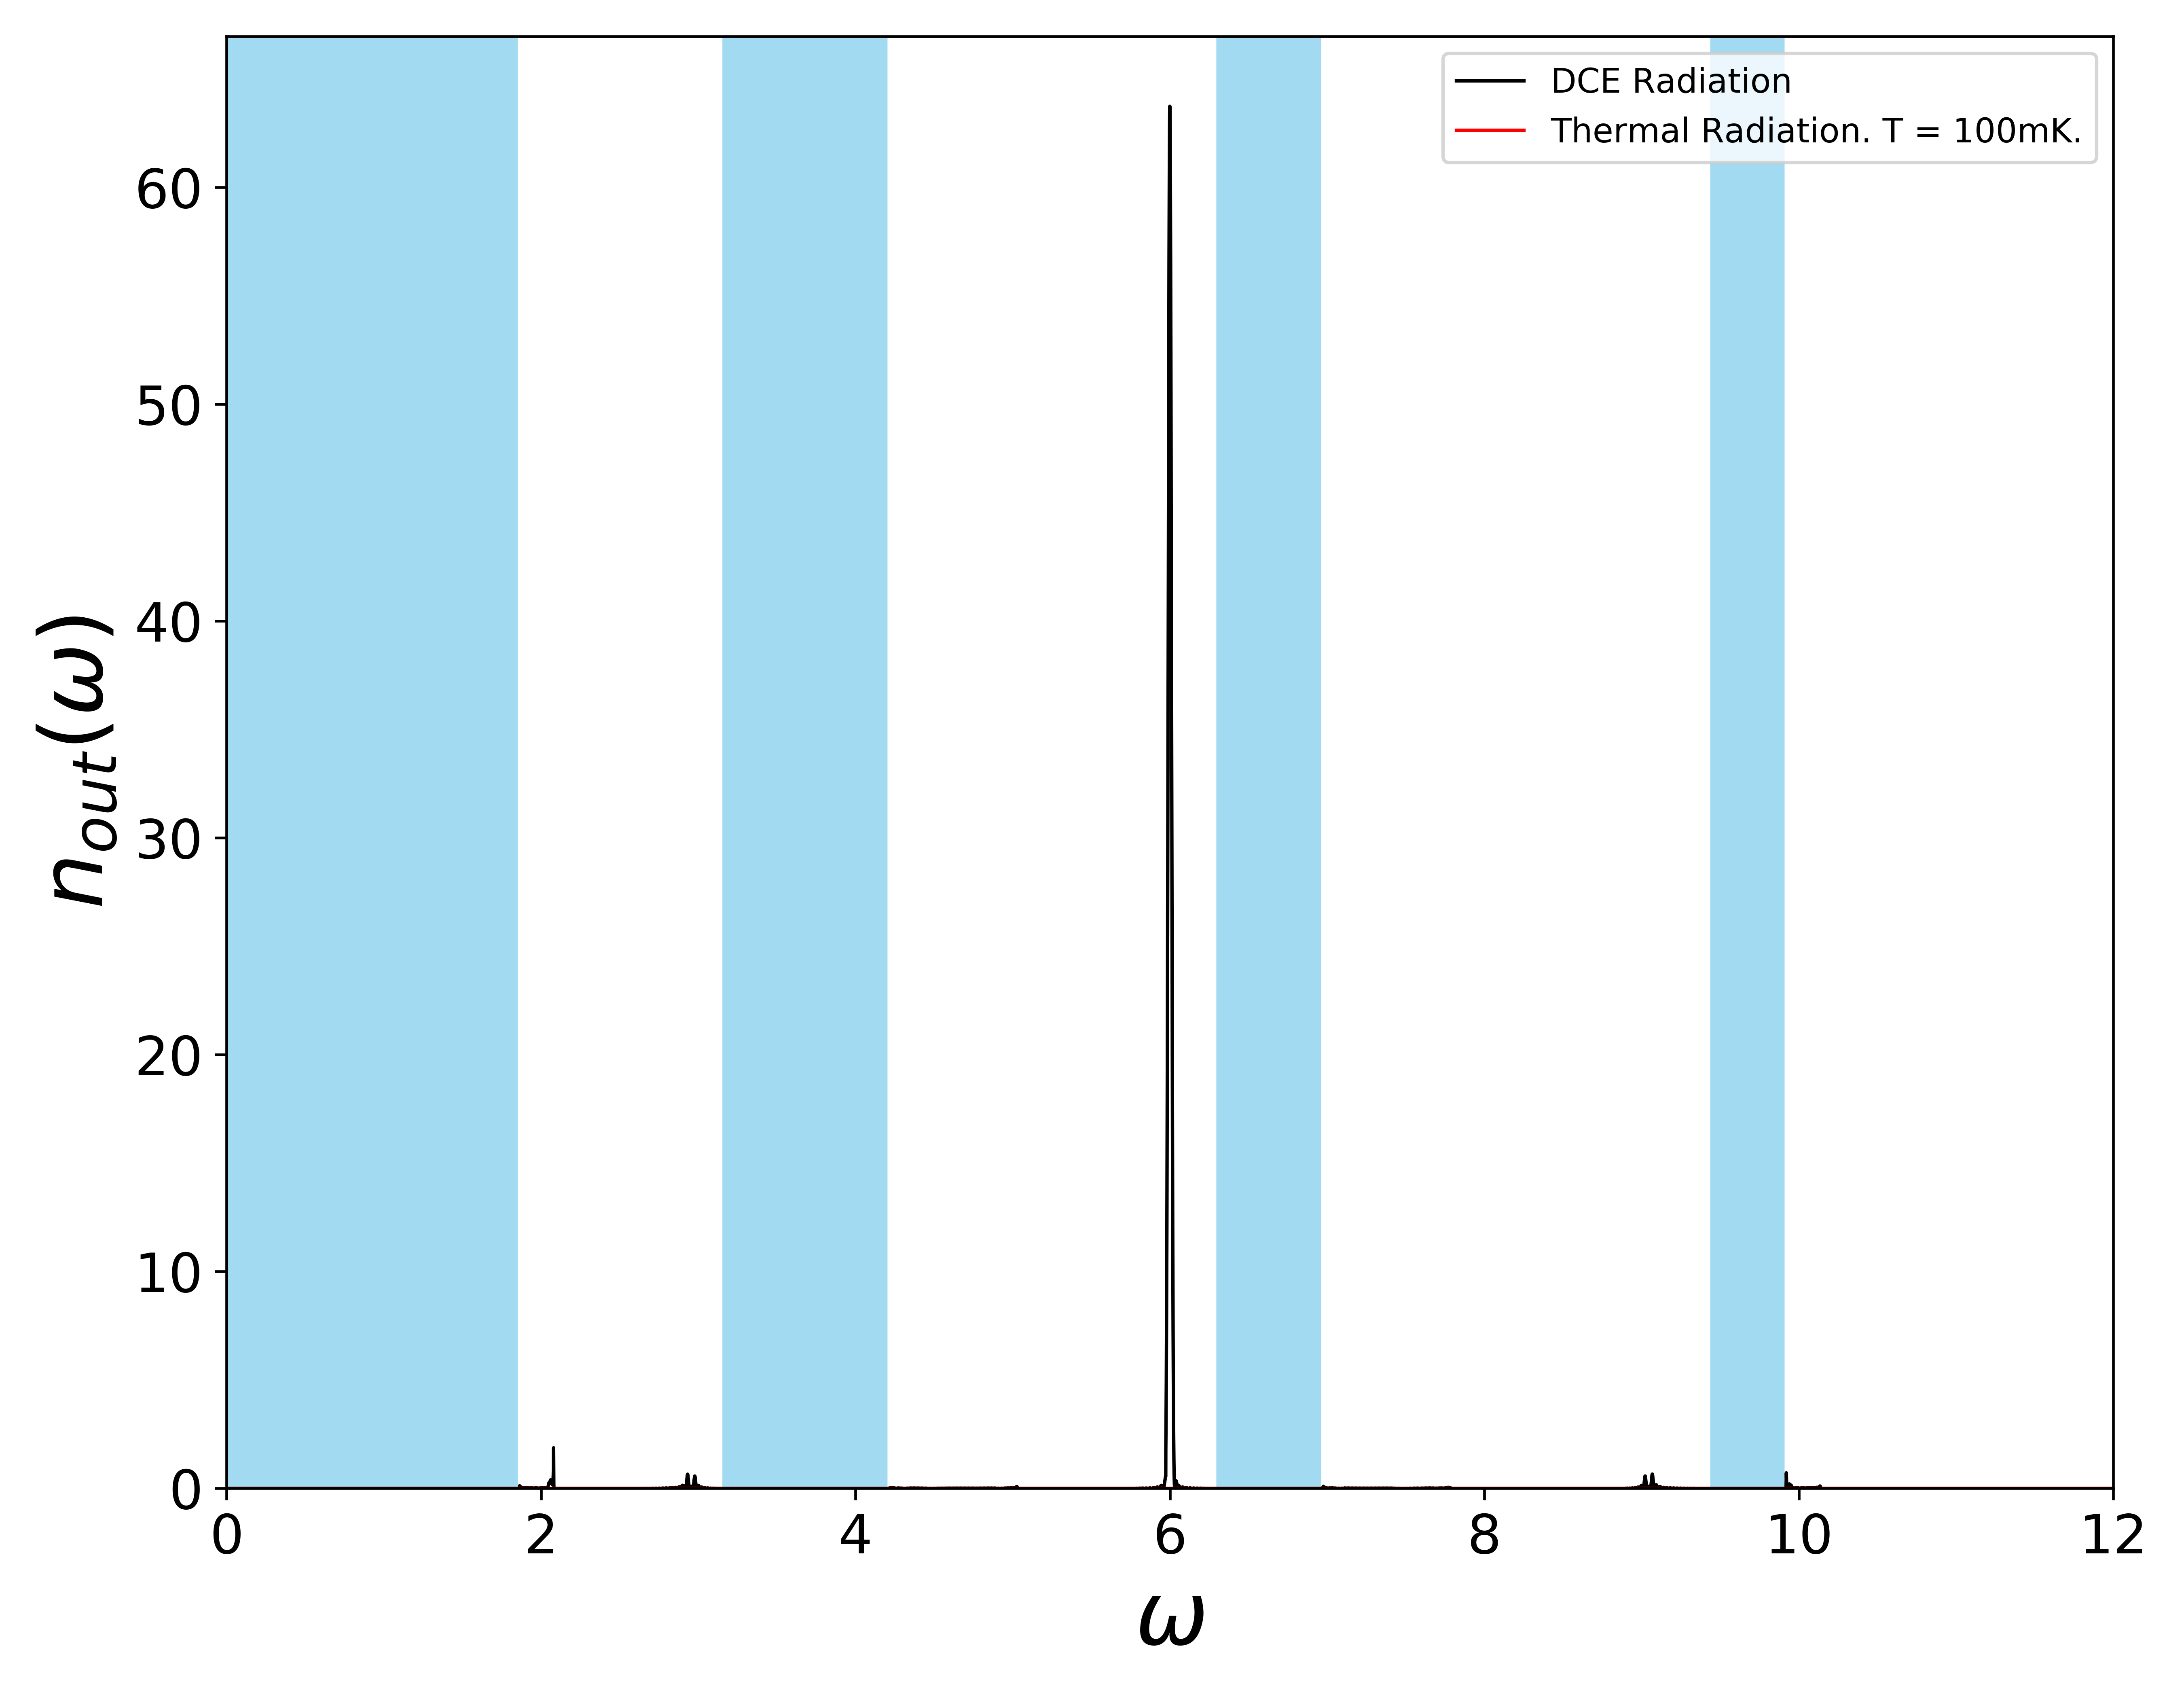
\includegraphics[width=\textwidth, keepaspectratio]{figures/results/100_SQUIDs_active_100mK.png}
    \caption{Output radiation for lattice of 100 driven SQUIDs. The frequency where most radiation is produced changes as we change number of SQUIDs.}
    \label{fig:100_SQUIDs_active}
\end{figure}

\clearpage
%
\begin{figure}[h]
    \centering
    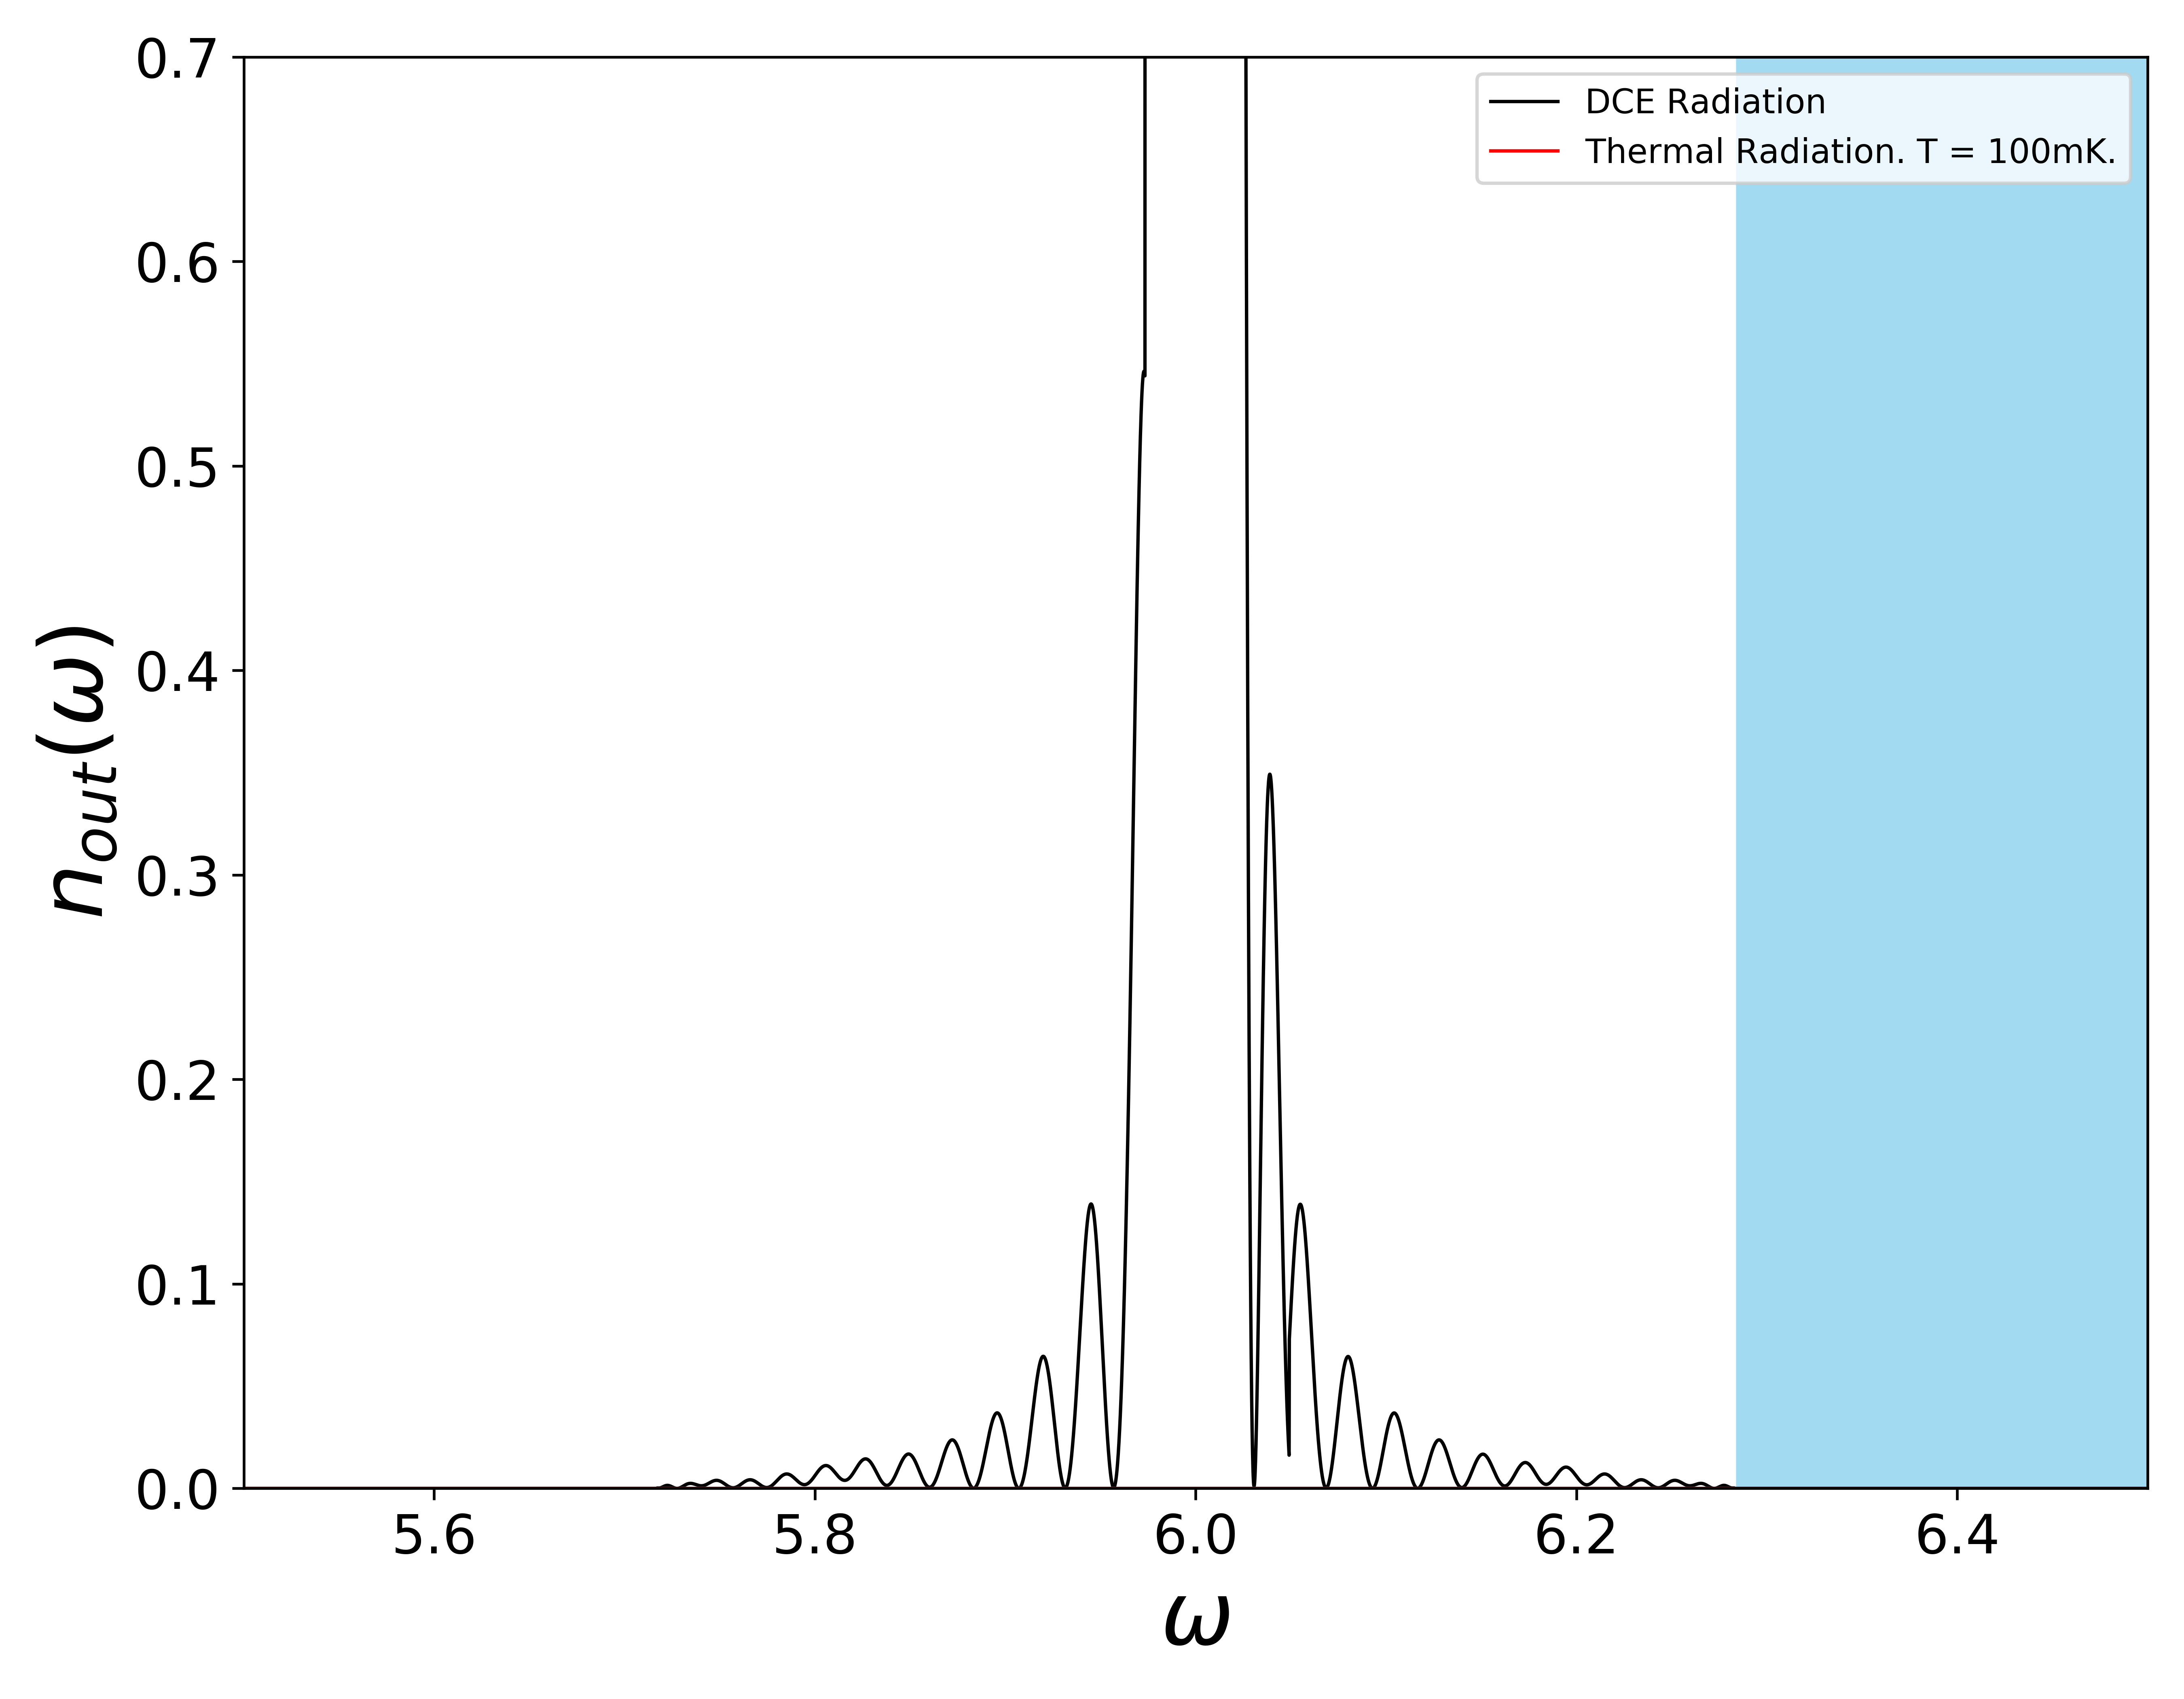
\includegraphics[width=\textwidth, keepaspectratio]{figures/results/100_SQUIDs_active_100mK_zoom.png}
    \caption{Output radiation for lattice of 100 driven SQUIDs. Here, we show the details of the radiation around half the oscillation frequency.}
    \label{fig:100_SQUIDs_active_zoomed}
\end{figure}
\clearpage
%

\begin{figure}[h]
    \centering
    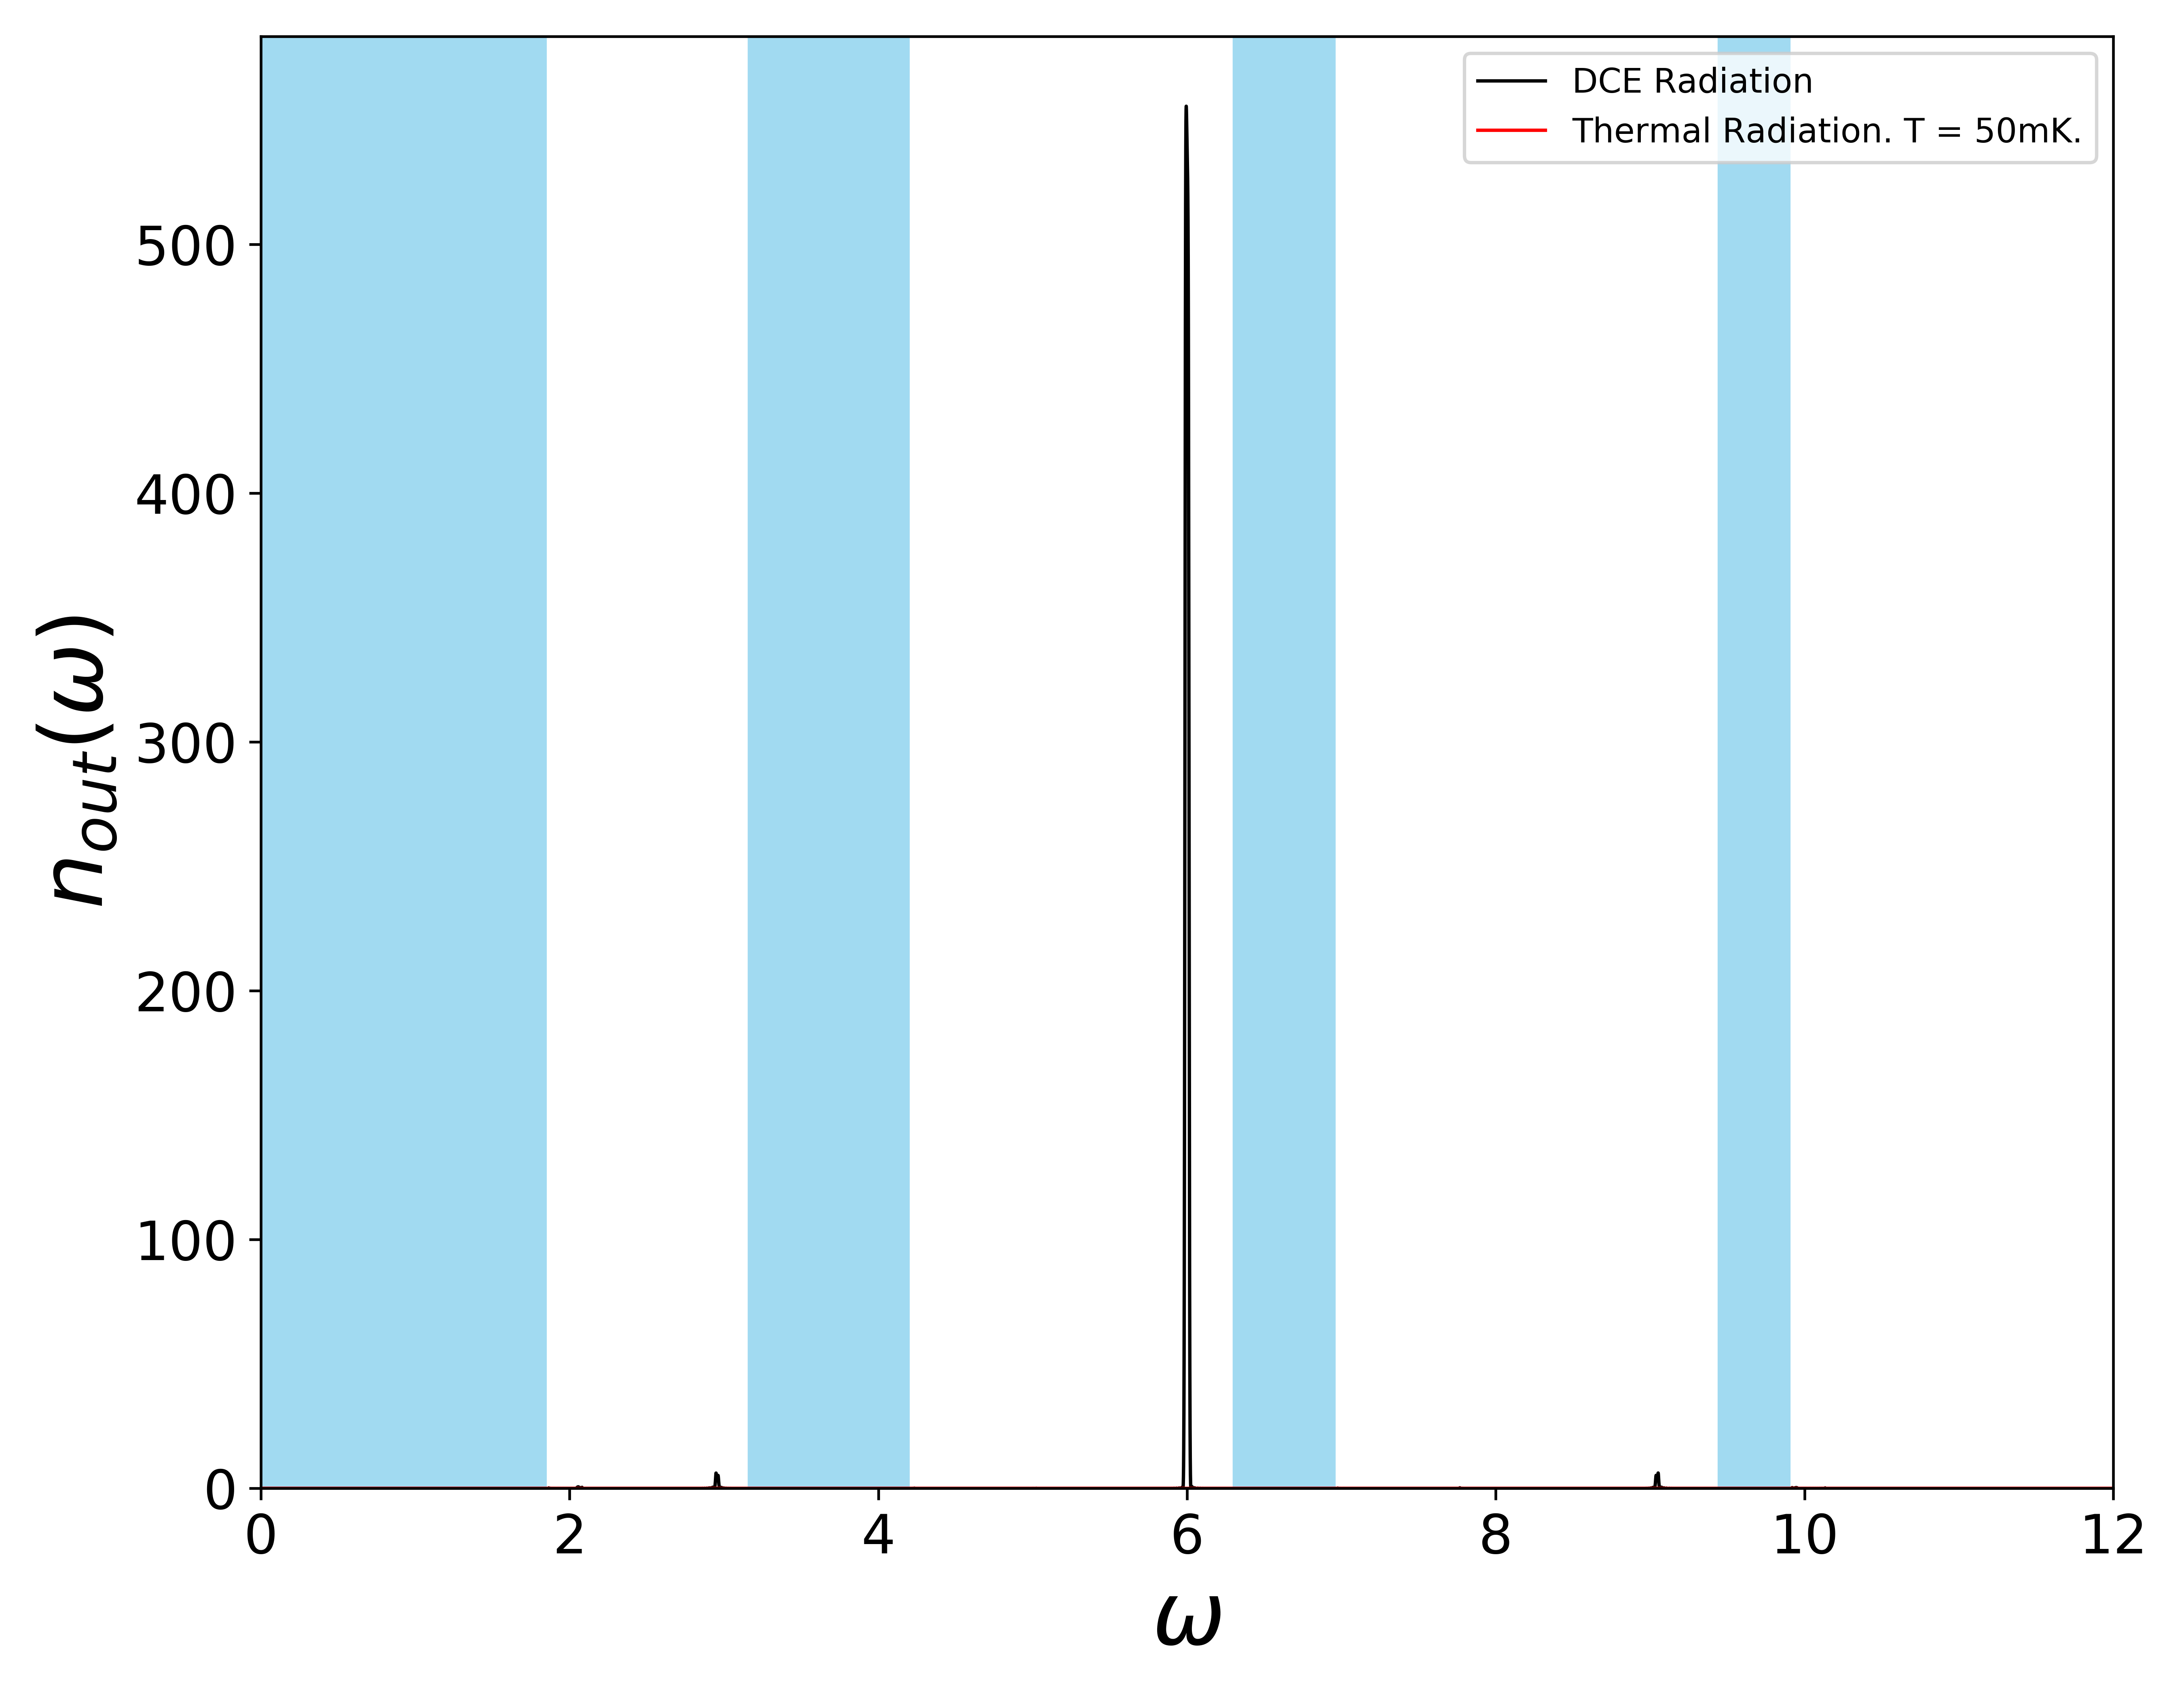
\includegraphics[width=\textwidth, keepaspectratio]{figures/results/150_SQUIDs_active.png}
    \caption{Output radiation for lattice of 150 driven SQUIDs. The magnitude of the photon-flux density changes in a non-trivial matter as we increase number of SQUIDs.}
    \label{fig:150_SQUIDs_active}
\end{figure}
\clearpage
%
%
\begin{figure}[h]
    \centering
    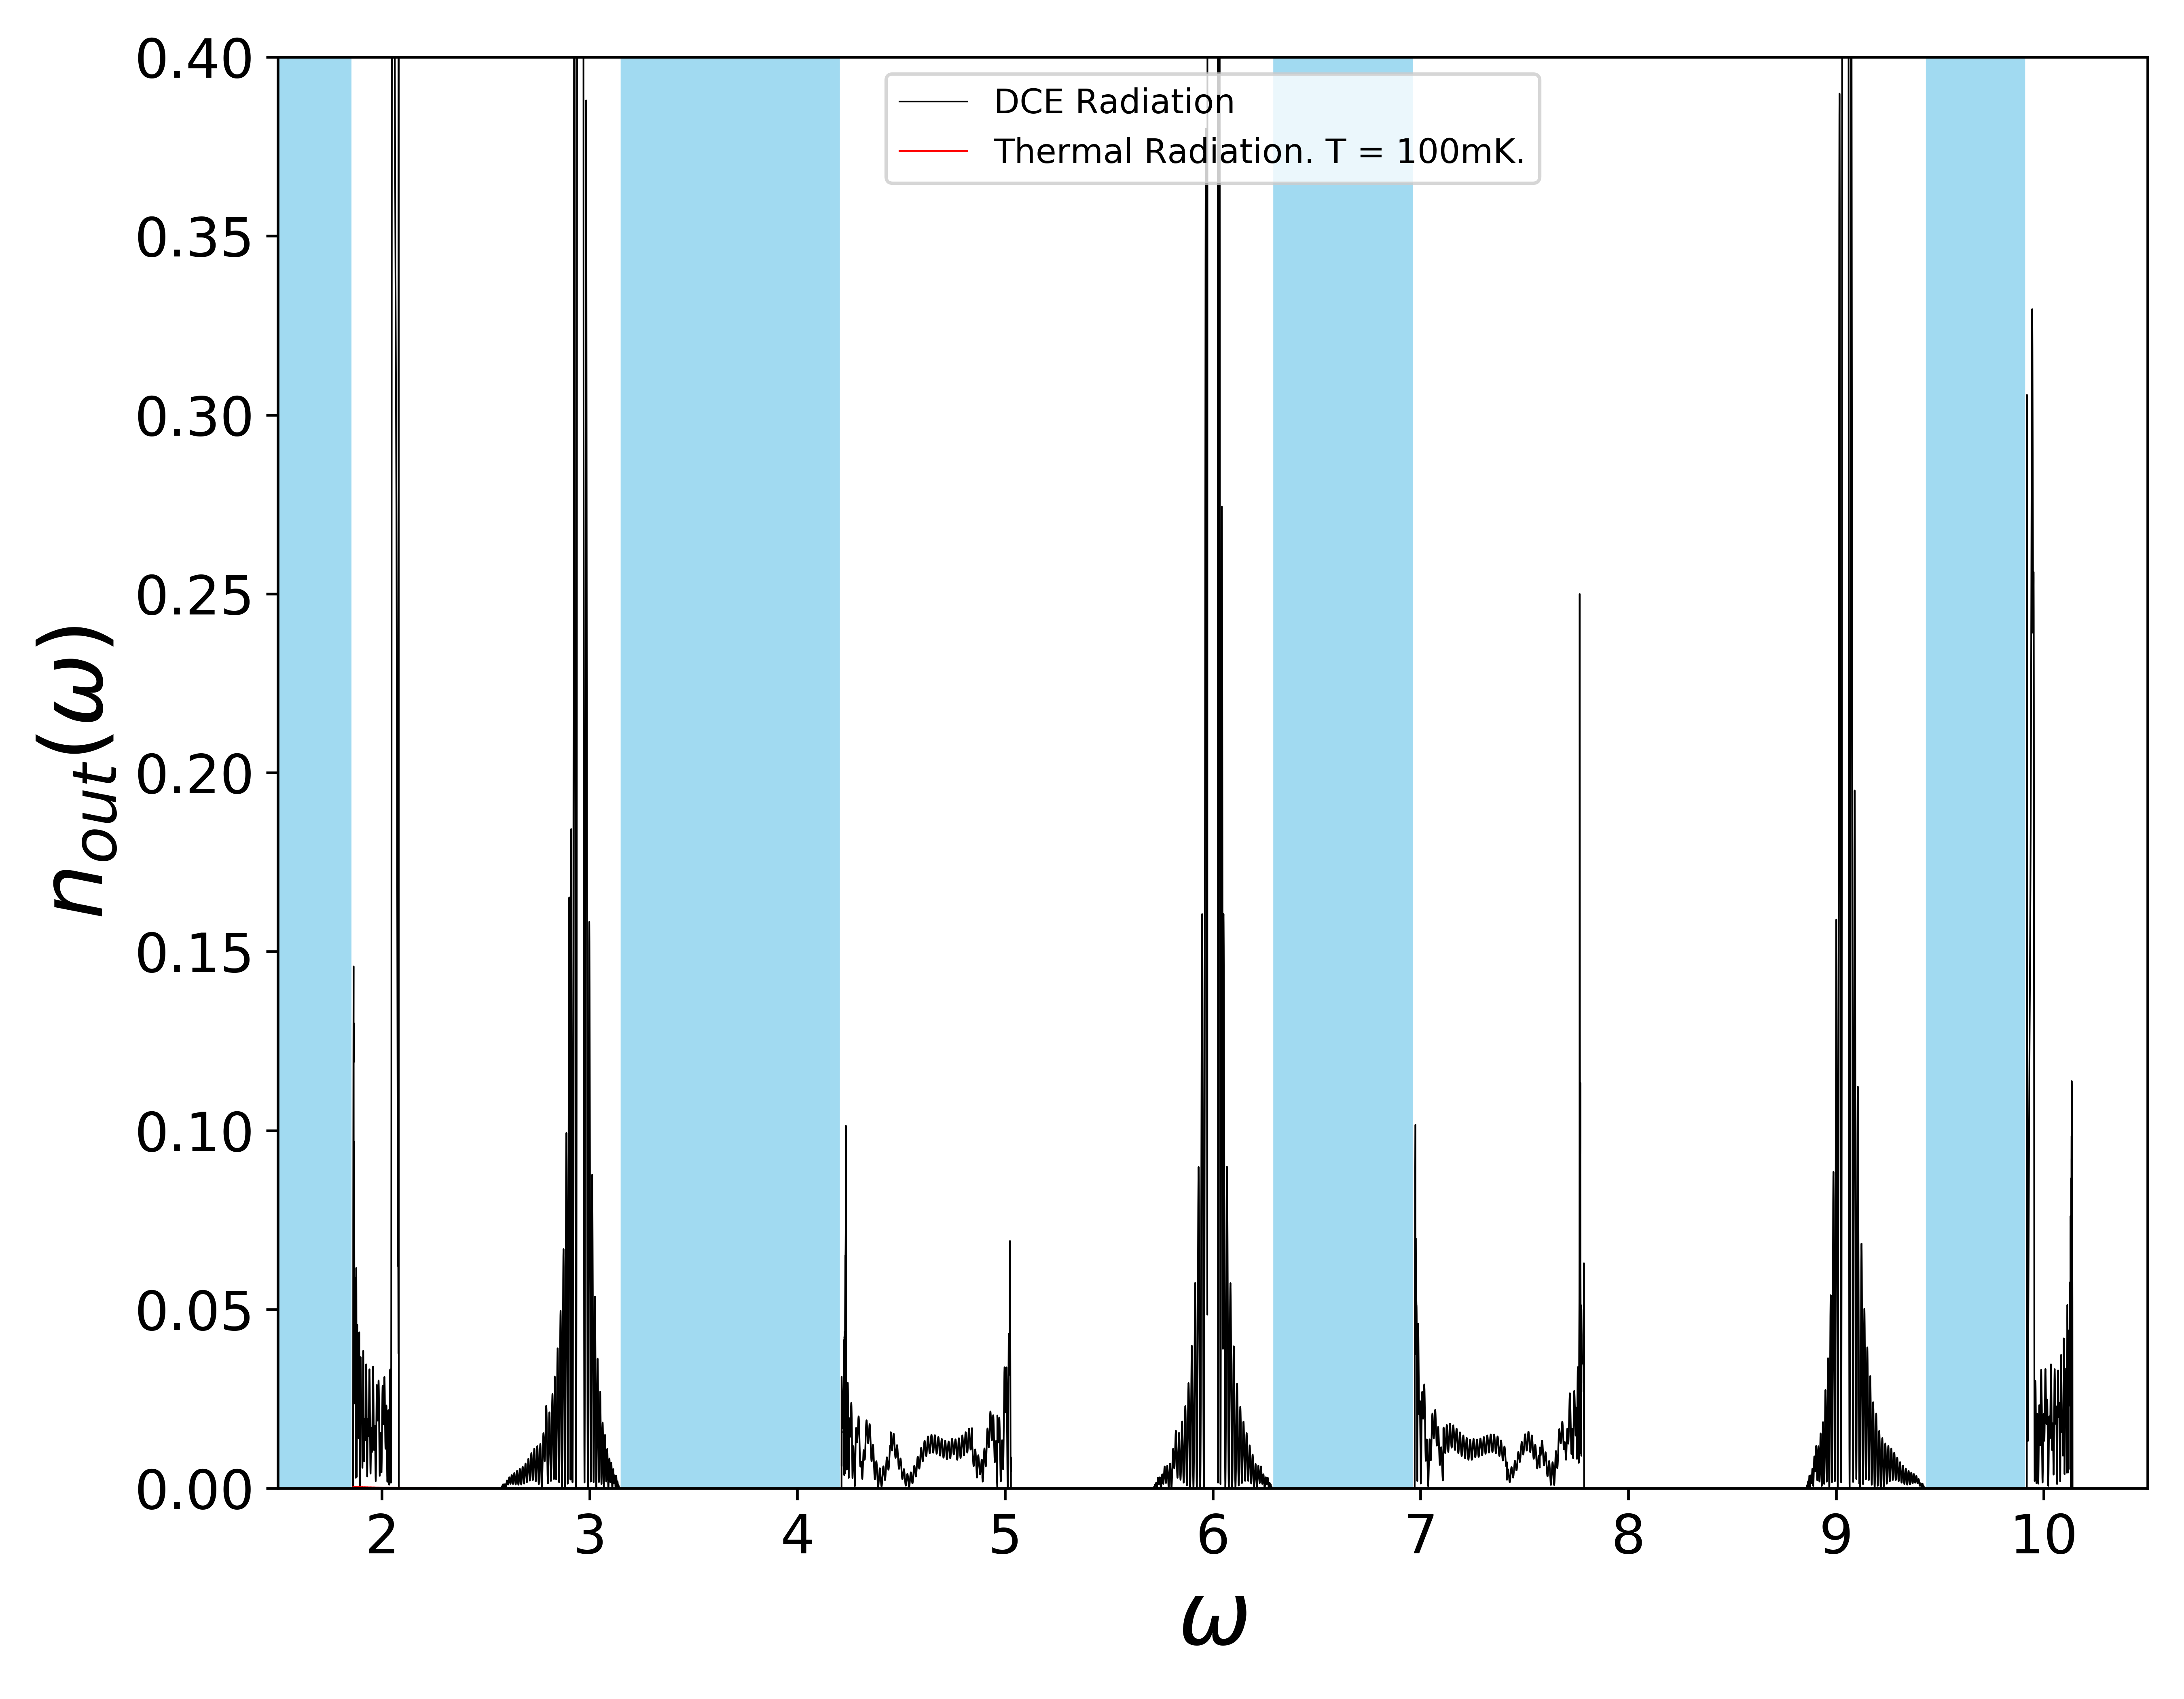
\includegraphics[width=\textwidth, keepaspectratio]{figures/results/150_SQUIDs_active_100mK_zoom.png}
    \caption{Output radiation for lattice of 150 driven SQUIDs. We show the detail in the behavior of photon production.}
    \label{fig:150_SQUIDs_active_zoomed}
\end{figure}
\clearpage
%

\section{Spatial symmetry breaking}\label{sec:results_symmetry_breaking}

For all of the previous results, the lattice had spatial symmetry, i.e., there was nothing distinguishing the left and right side. Thus, the radiation emitted from each side was equal. We now turn our attention to a lattice of driven SQUIDs with a site dependent phase $\varphi_n$. By implementing this phase factor, we break the spatial symmetry and obtain different radiation spectra emitted from different sides of the lattice.
%
\begin{figure}[h]
    \centering
    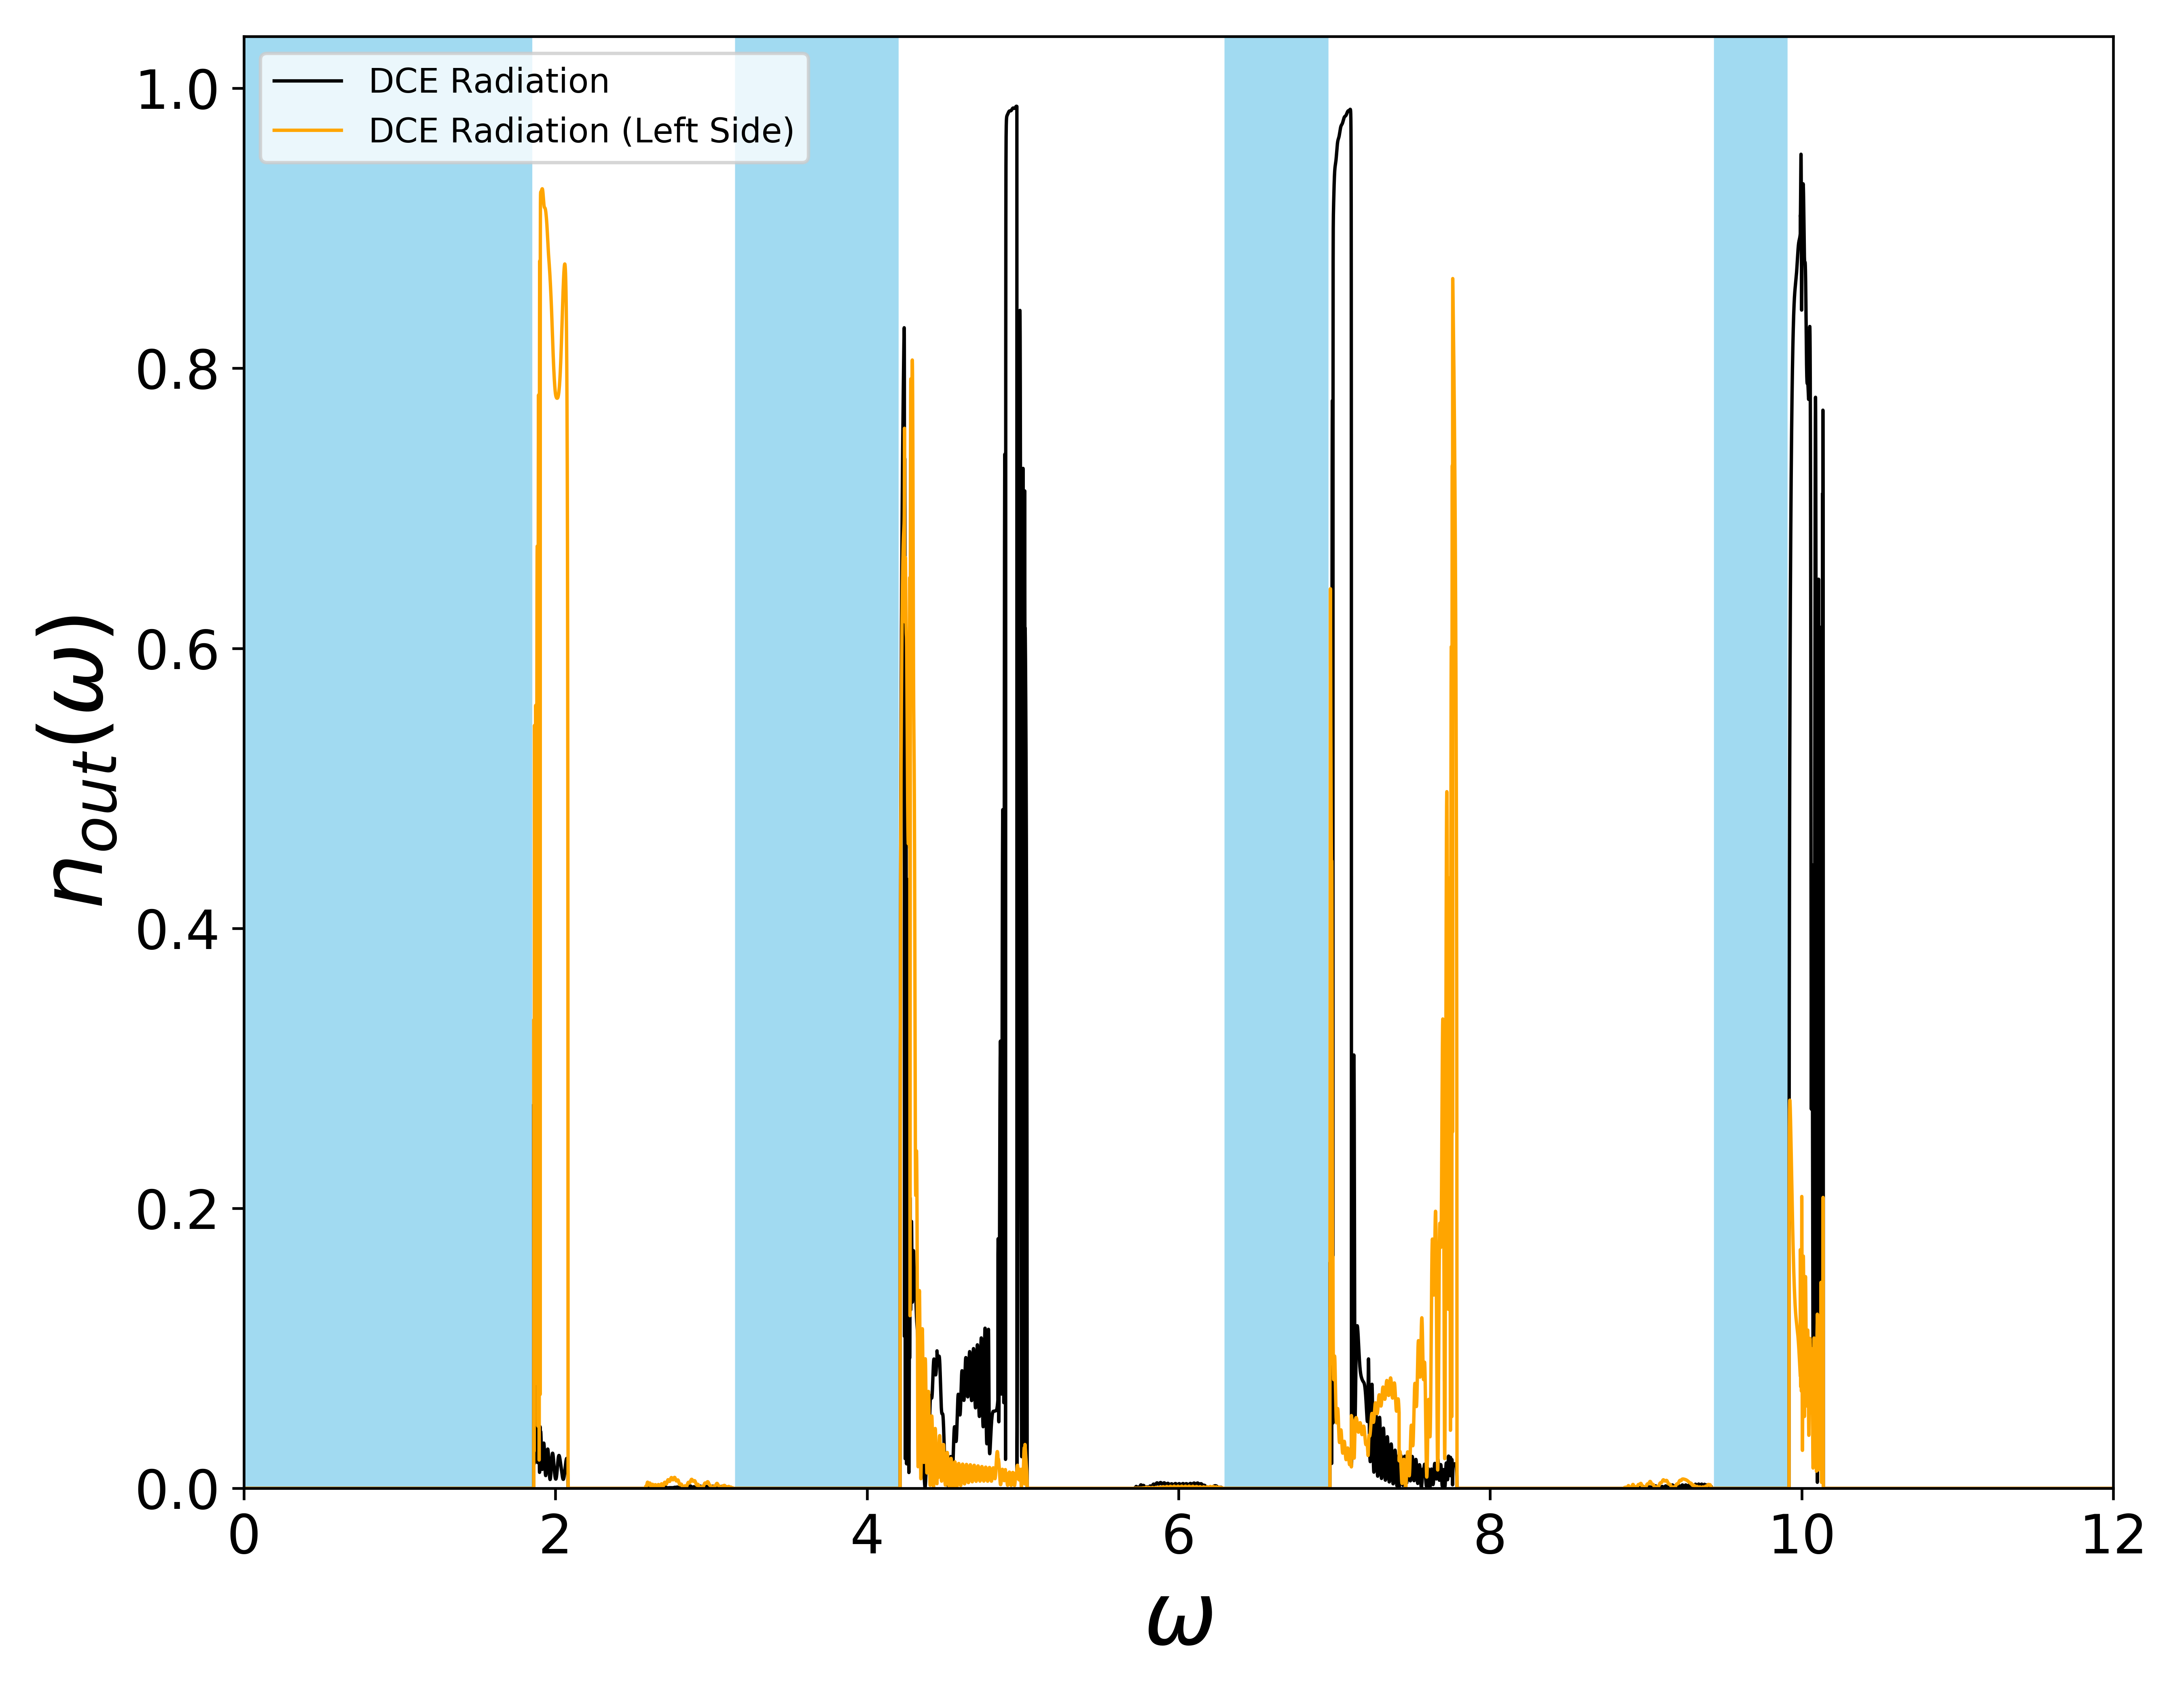
\includegraphics[width=\textwidth, keepaspectratio]{figures/results/phase_shift_2pi_3_both.png}
    \caption{Output radiation for lattice of 100 SQUIDs driven out of phase. Introducing a phase shift factor breaks the spatial symmetry of the lattice. Here, each SQUID is driven at a phase difference of $\frac{2\pi}{3}$ with respect to the previous SQUID, effectively creating a new 3-SQUID unit cell.}
    \label{fig:phase_2pi_3_both}
\end{figure}
\clearpage
%
%
\begin{figure}[h]
    \centering
    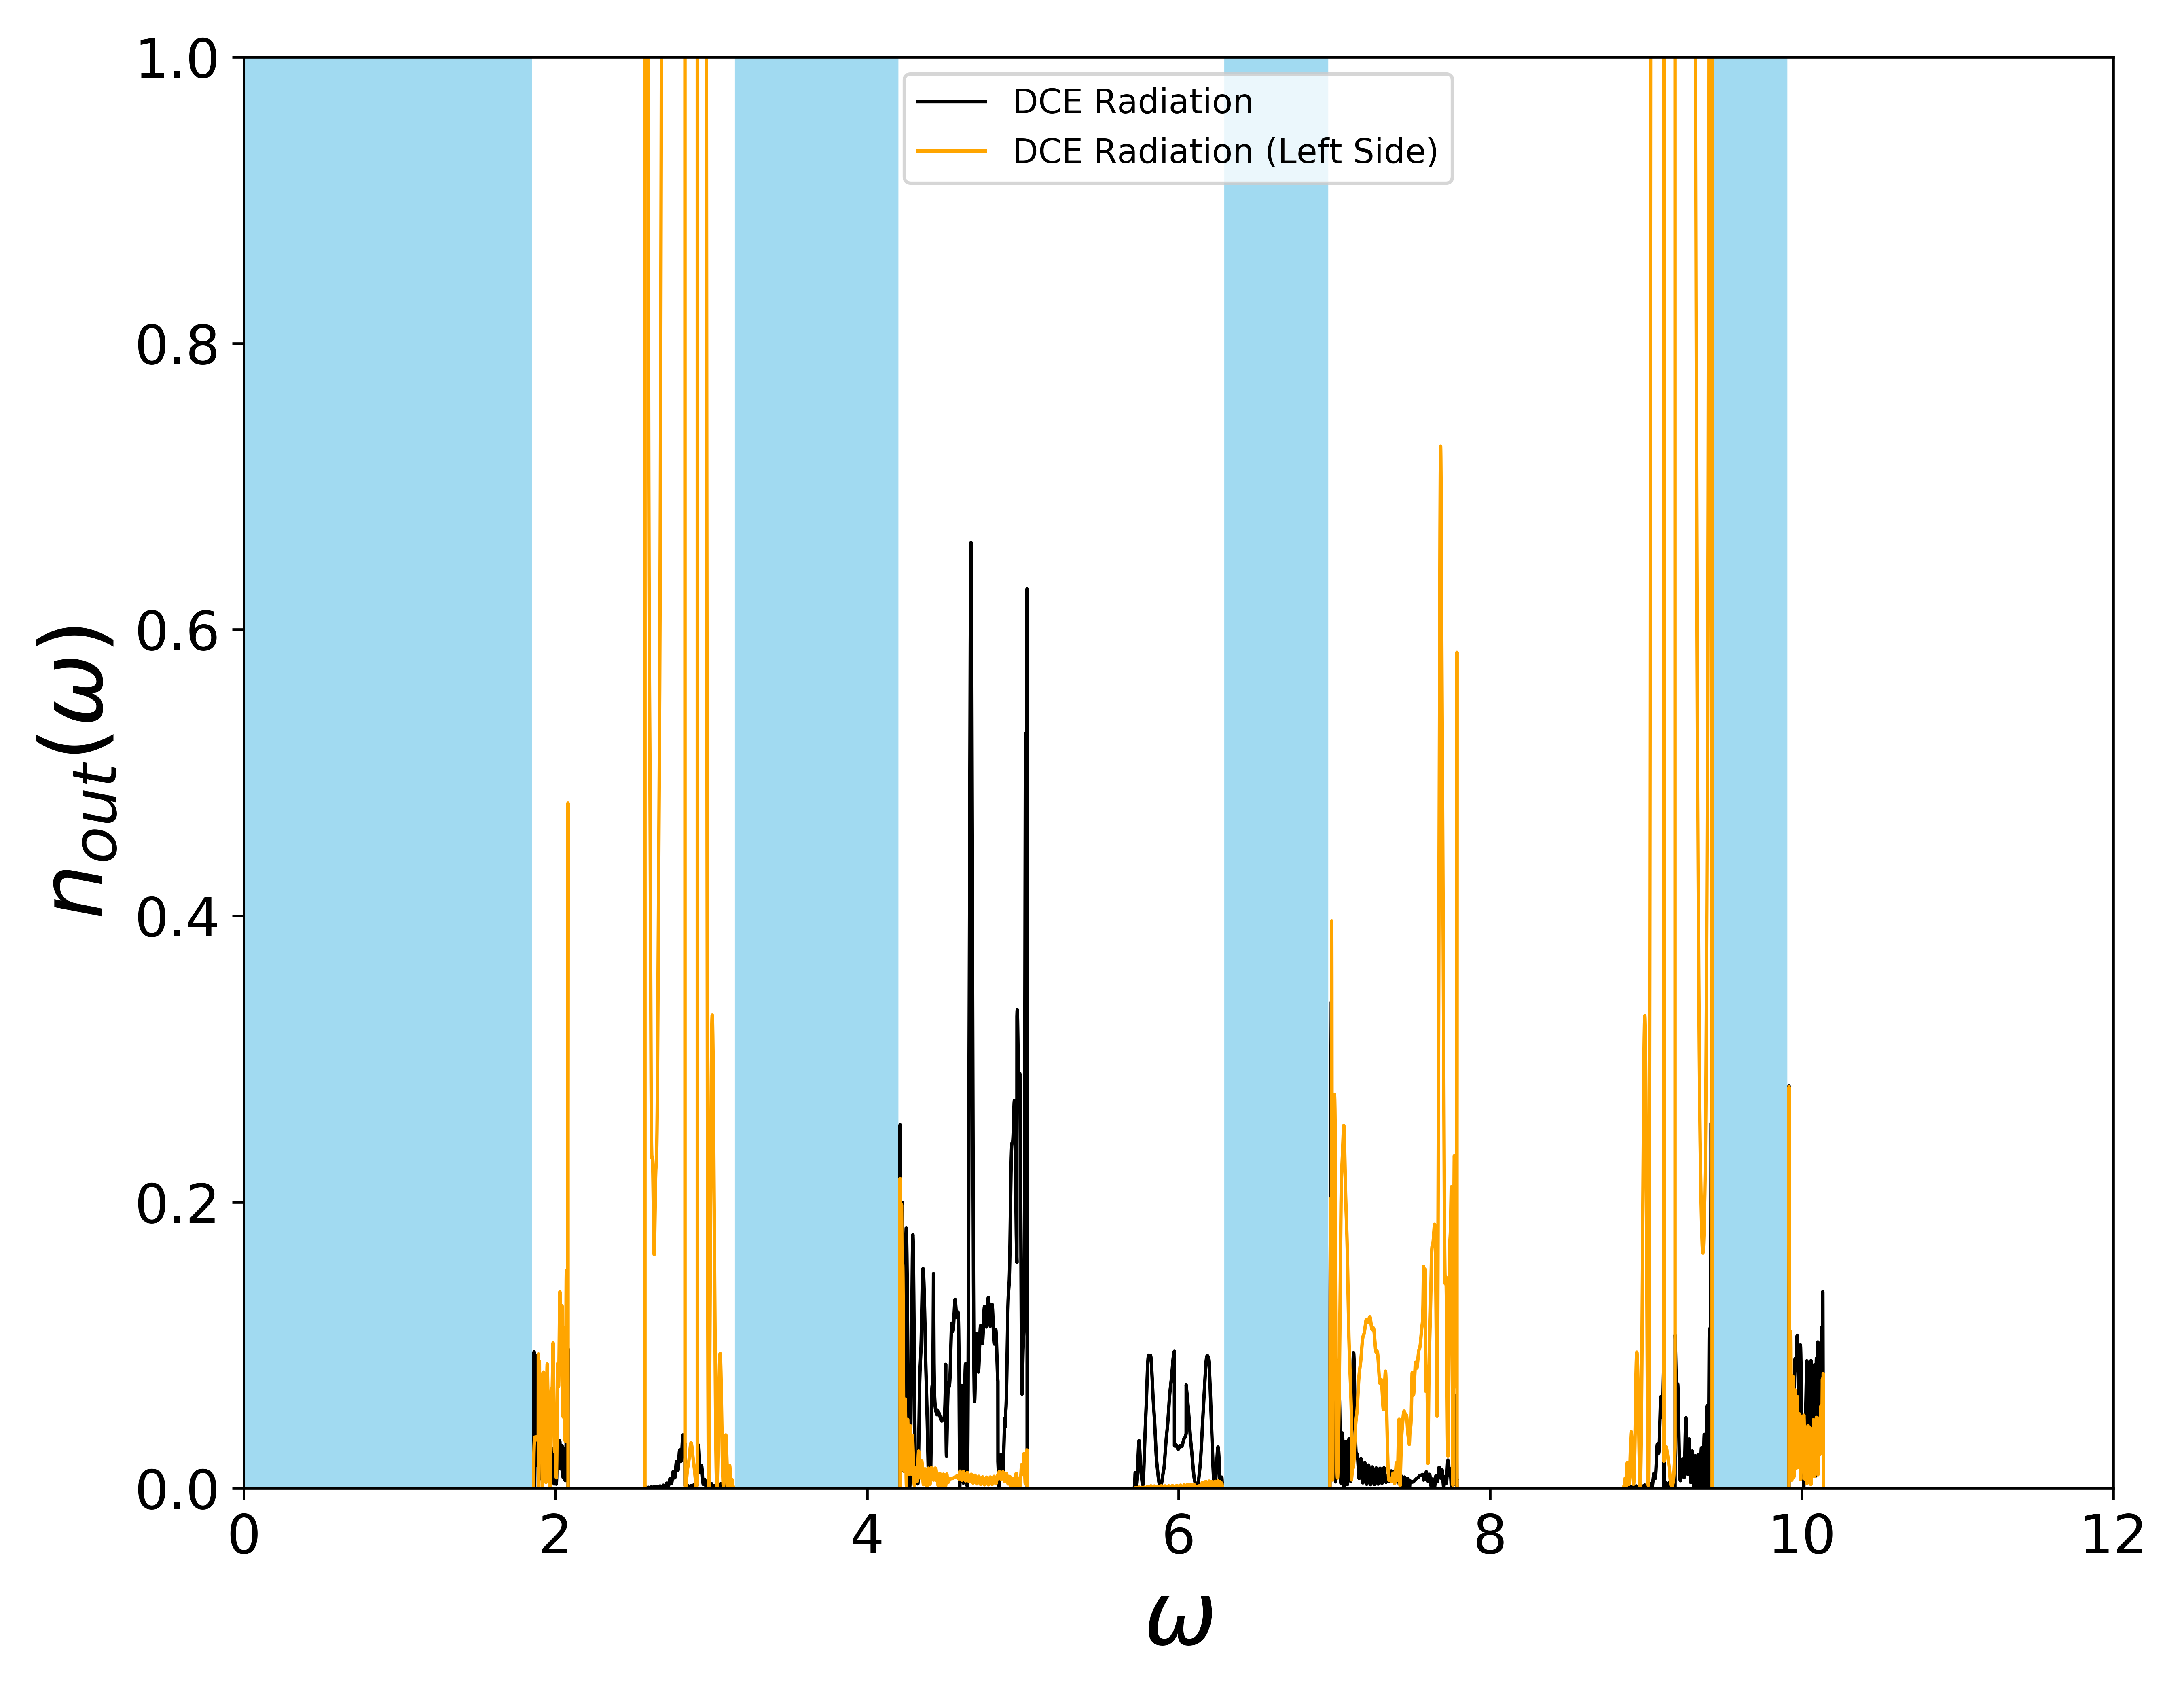
\includegraphics[width=\textwidth, keepaspectratio]{figures/results/phase_shift_2pi_5_both_zoom.png}
    \caption{Output radiation for lattice of 100 SQUIDs driven out of phase. Phase factor = $\frac{2\pi}{5}$, 5-SQUID unit cell. Our system is highly susceptible to changes in phase.}
    \label{fig:phase_2pi_5_both}
\end{figure}
\clearpage
%
\begin{figure}[h]
    \centering
    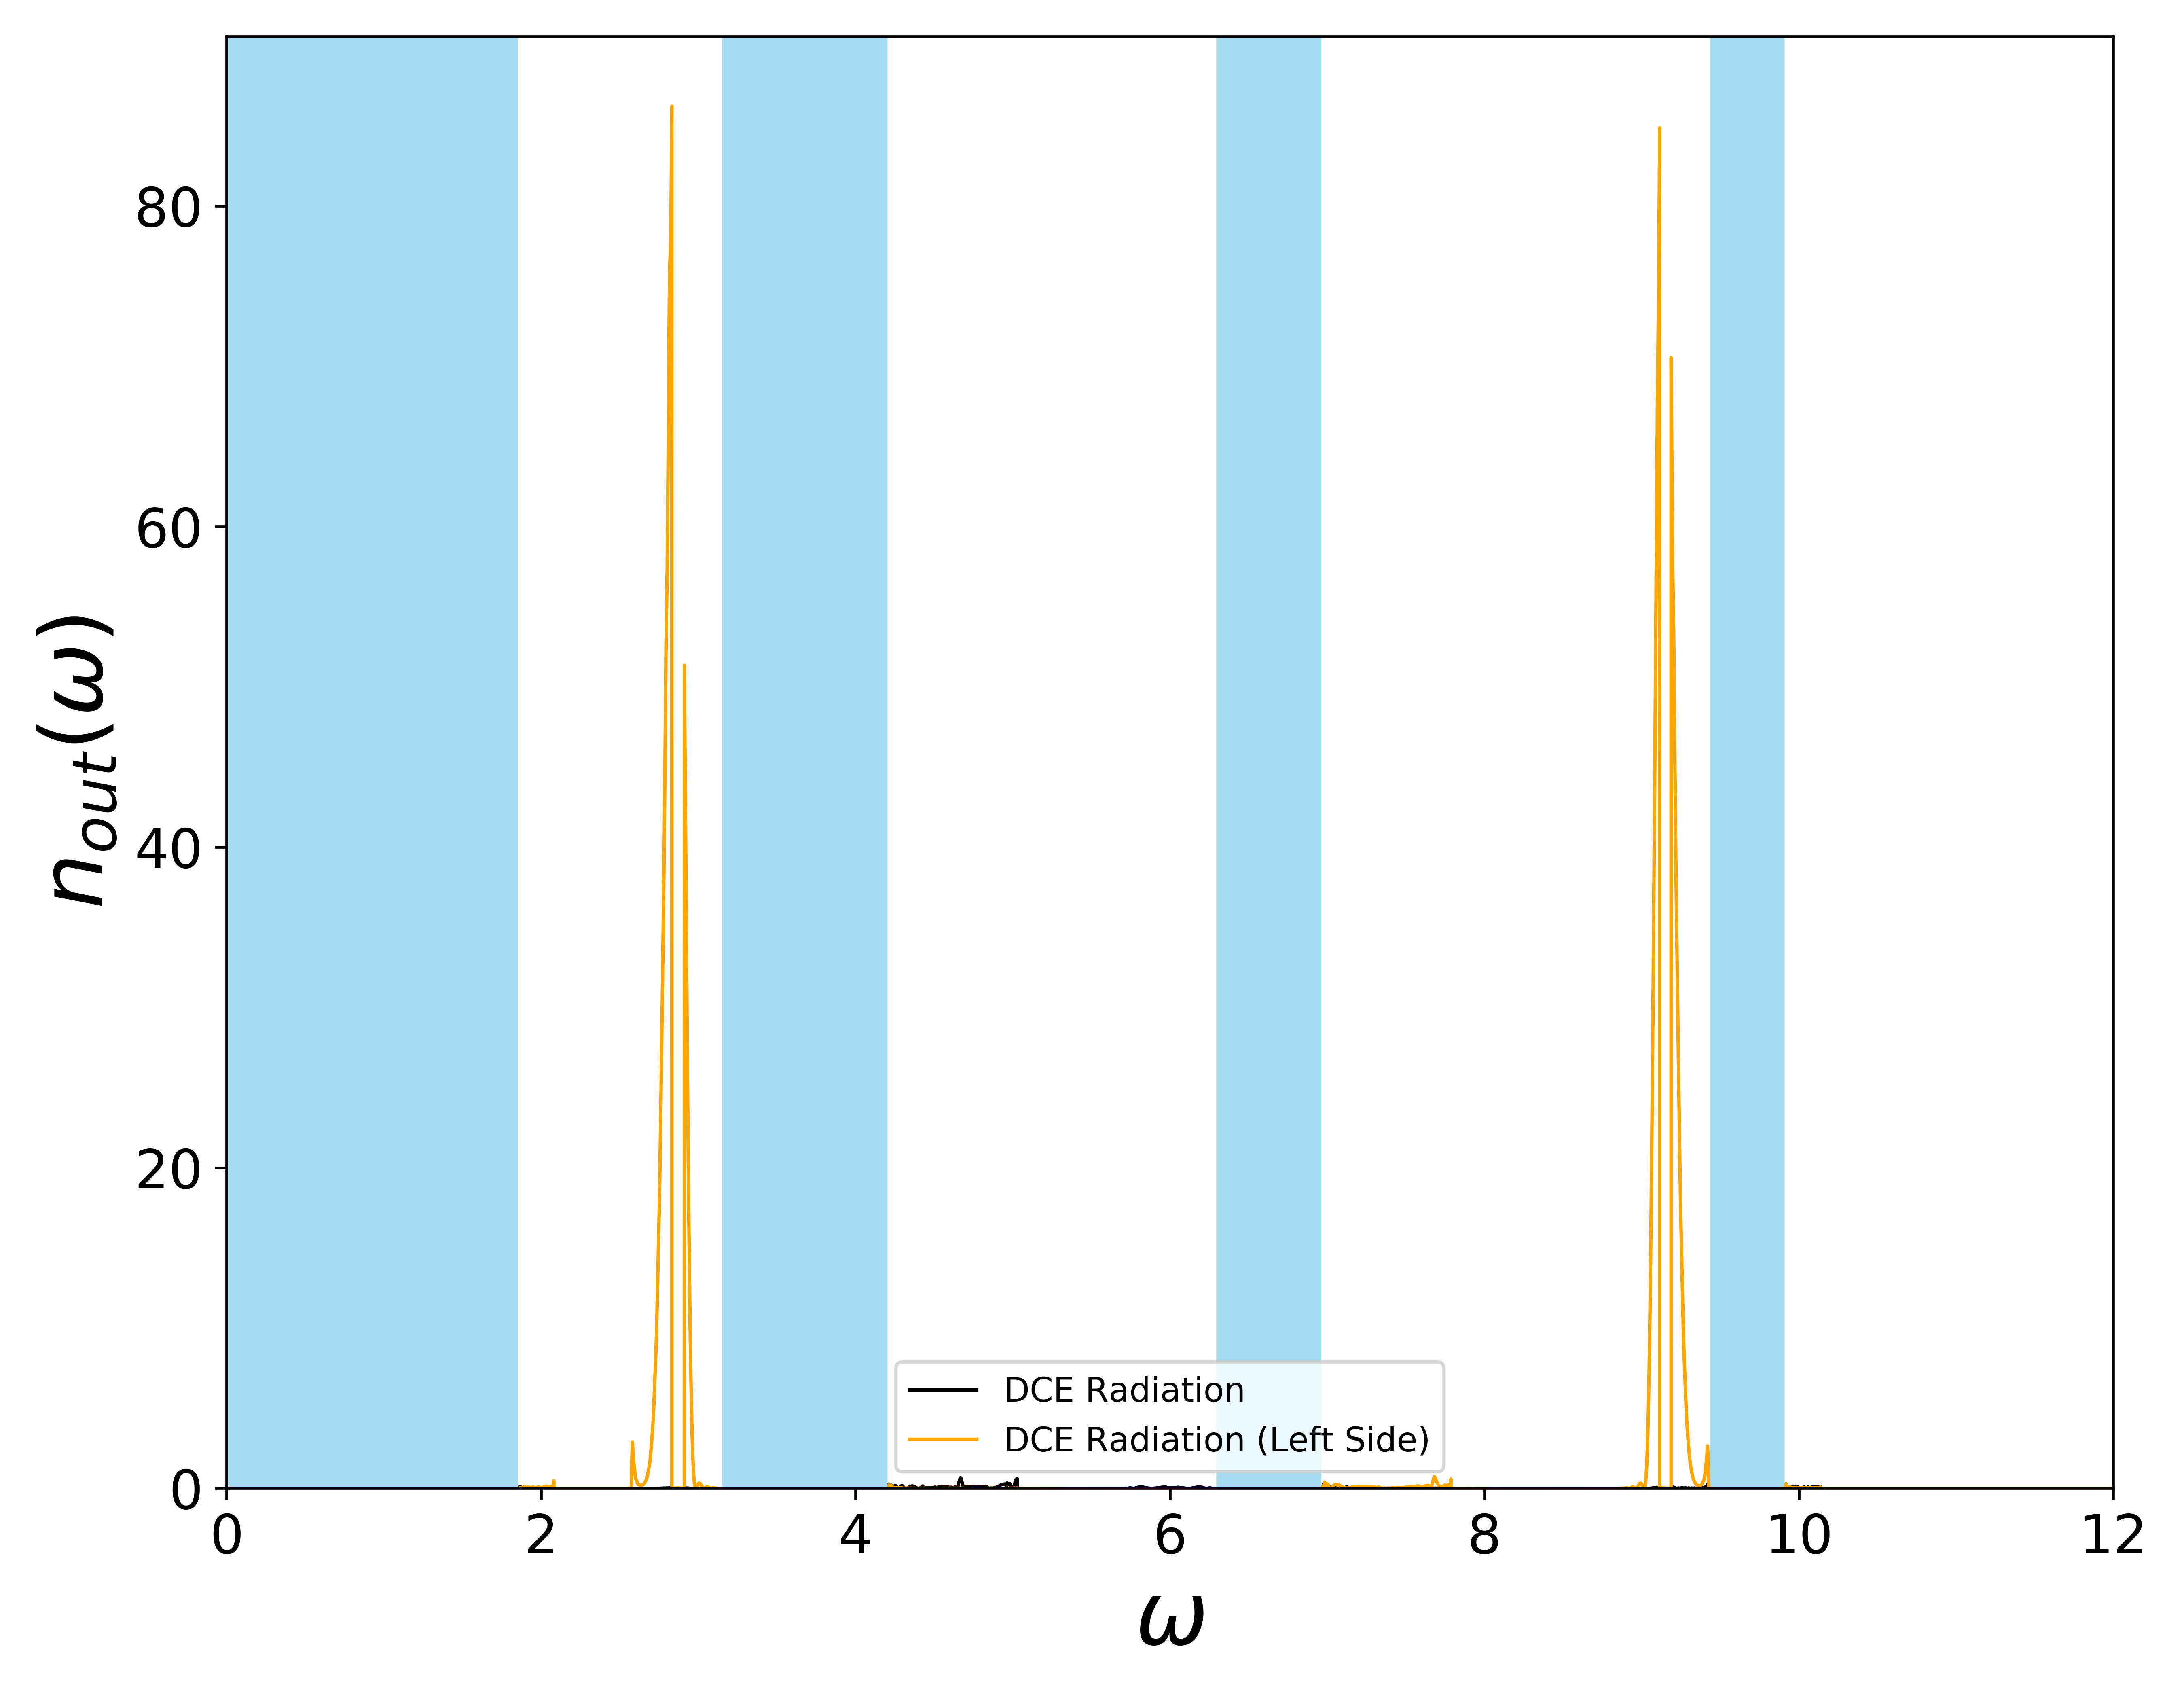
\includegraphics[width=\textwidth, keepaspectratio]{figures/results/phase_shift_2pi_5_both.png}
    \caption{Output radiation for lattice of 100 SQUIDs driven out of phase. Phase factor = $\frac{2\pi}{5}$, 5-SQUID unit cell. Drastic difference in the left/right output radiation (quasi-unidirectionality) is achieved.}
    \label{fig:phase_2pi_5_both_zoomed}
\end{figure}
\clearpage
\section{Final Remarks}\label{sec:remarks}

We have proposed a new system in which to study the dynamical Casimir effect, as well developed a theoretical and computational model its behaviour. The resulting model exhibits non-trivial features like the presence of a band structure, and the particular way in which the DCE scattering process occur in this band structure.
Moreover, the system is quite versatile. The band structure can be tuned by changing the spatial distance $\ell$ between SQUIDs, as well as their Josephson energy $E_J^0$ (which corresponds to changing the strength of the potential at each site). The harmonic drive of the SQUIDs generating the DCE radiation can be tuned in terms of the drive frequency $\Omega$, amplitude $\delta E_{J,\,n}$, and phase $\varphi_n$, where the latter two parameters can be modulated for each SQUID $n$ in the periodic array individually. This allows us to control spectral and spatial properties of the dynamical Casimir light emitted. We find a rich interplay between the band structure of the lattice, the harmonic drive of the SQUIDs, and the DCE photon-flux density, which thus allows us to control, guide, and manipulate DCE radiation. 
